\documentclass[11pt, a4paper, titlepage]{scrreprt}

\usepackage[latin1]{inputenc}
\usepackage[english]{babel}
\usepackage{graphicx}
\usepackage{booktabs}
\usepackage{geometry}
\usepackage{setspace}
\usepackage{fancyhdr}
\usepackage{url}
\usepackage{wrapfig}
\usepackage[usenames,dvipsnames]{color}
\usepackage{colortbl}
\usepackage{eso-pic}
\usepackage{listings}
\usepackage{fix-cm}
\usepackage{textcomp}
\usepackage[T1]{fontenc}


%\usepackage[automark]{scrpage2}
%\usepackage[absolute]{textpos}

\lstset{language=[Sharp]C, % base language is C and dialect is Sharp (C#)
captionpos=b, % descriptions are underneath
frame=lines, % above und underneath the code listing are horizontal lines
basicstyle=\ttfamily, % font
keywordstyle=\color{blue}, % Color for keywords like public, void, object, etc.
commentstyle=\color{ForestGreen}, % Color for comments
stringstyle=\color{BrickRed}, % Color for strings
numbers=left, % line numbers to the left of the code
numberstyle=\tiny, % small line numbers
numbersep=5pt,
tabsize=2,
breaklines=true, % Wordwrap activated
showstringspaces=false,
morestring=[b]', % counts single quote pairs as strings (and thus also colors them red)
upquote=true, % changes smart single quotes to straight ' marks
% emph defines certain colors for specific words
% emph={double,bool,int,unsigned,char,true,false,void},emphstyle=\color{blue},
emph={Assert,Test}, emphstyle=\color{BrickRed},
emph={[2]double,bool,int,unsigned,char,true,false,void,using,\#define,\#ifdef,\#endif,\#region,\#endregion},
emphstyle={[2]\color{blue}}
}

\geometry{a4paper, portrait, left=2cm, right=2cm, top=2cm, bottom=2cm, includefoot}

%\pagestyle{headings}
%\pagestyle{scrheadings}
\pagestyle{fancy} % self-made page style
\fancyhf{} % clear all header and footer fields
\fancyhead[L]{\leftmark} % left header
\fancyhead[C]{\AddToShipoutPicture*{\BackgroundHeaderPic}} % center header
%\fancyhead[R]{\rightmark} % right header --> Removed because it overflows on the leftmark if the text is too long

\fancyfoot[C]{\thepage\AddToShipoutPicture*{\BackgroundFooterPic}} % center footer
%\fancyfoot[EL,OR]{\thepage} % page number
%\fancyfoot[ER,OL]{
\includegraphics[height=0.3cm]{figures/ct_logo}}

\renewcommand{\headrulewidth}{2pt} % upper separator
\renewcommand{\footrulewidth}{2pt} % lower separator

\newlength{\headbgwidth}
\setlength{\headbgwidth}{\headwidth}
%\addtolength{\headbgwidth}{0.3mm}
%\addtolength{\headwidth}{\marginparwidth}


\renewcommand{\headrule}{{\color{orange}\hrule width\headwidth height\headrulewidth \vskip-\headrulewidth}}
\renewcommand{\footrule}{{\color{orange}\vskip-\footruleskip\vskip-\footrulewidth\hrule width\headwidth height\footrulewidth\vskip\footruleskip}}


\makeatletter
\newcommand\BackgroundHeaderPic{
%\AddToShipoutPicture{%
    \setlength{\@tempdimb}{1.87cm}%
    \setlength{\@tempdimc}{28.4cm}%
    \setlength{\unitlength}{1pt}%
    \put(\strip@pt\@tempdimb,\strip@pt\@tempdimc){
        
\includegraphics[width=\headbgwidth, height=\headheight]{figures/ct_page_header}%
    }
}

\newcommand\BackgroundFooterPic{
%\AddToShipoutPicture{%
    \setlength{\@tempdimb}{1.87cm}%
    \setlength{\@tempdimc}{1.8cm}%
    \setlength{\unitlength}{1pt}%
    \put(\strip@pt\@tempdimb,\strip@pt\@tempdimc){
        
\includegraphics[width=\headbgwidth, height=0.7cm]{figures/ct_page_footer_pure}%
    }
}

\newcommand\WaterMarkPic{%
    \setlength{\@tempdimb}{1.85cm}%
    \setlength{\@tempdimc}{2.7cm}%
    \setlength{\unitlength}{1pt}%
    \put(\strip@pt\@tempdimb,\strip@pt\@tempdimc){
            
\includegraphics[width=0.6\textwidth]{figures/ct_logo_watermark}%
    }
}
\makeatother

% finetune the gaps between figure and text in the subfigure environment (basically close the gap as much as possible)
%\renewcommand{\subfigtopskip}{0pt}
%\renewcommand{\subfigbottomskip}{0pt}

% some color definitions for the pdf statements below
\definecolor{mygrey}{rgb}{0.45,0.45,0.45}
\definecolor{mydarkgrey}{rgb}{0.2,0.2,0.2}
\definecolor{red}{rgb}{1.0,0.33,0.33}
\definecolor{orange}{rgb}{1.00,0.73,0.33}
\definecolor{yellow}{rgb}{0.95,0.92,0.}
\definecolor{lightgreen}{rgb}{0.3,0.95,0.46}
\definecolor{titleblue}{rgb}{0.03,0.10,0.46}


% requires the following:
% \usepackage[absolute]{textpos}
\begin{titlepage}
\vspace*{-1cm}
\newlength{\links}
\setlength{\links}{0.9cm}
\setlength{\TPHorizModule}{1cm}
\setlength{\TPVertModule}{1cm}
\textblockorigin{0pt}{0pt}

\sf
\LARGE

\begin{textblock}{14.5}(3.2,6.5)
\Large [fancy logo] \\[3cm]  
{ \bf CrypTool 2.0} \\[1cm]
{\LARGE \bf DEVELOPER INFORMATION}\\[1.3cm]

\normalsize Authors:\\
\Large Sebastian Przybylski\\
etc.\\

\large \today\\
Version 0.1
\end{textblock}

\end{titlepage}



\title{Plugin Developer Manual}
\subtitle{How to build your own plugins for CrypTool 2.0}
\author{S.\ Przybylski, A.\ Wacker, M.\ Wander, F.\ Enkler and P.\ Vacek}
\email{\{przybylski$|$wacker$|$wander$|$enkler$|$vacek\}@cryptool.org}
\version{0.5}
\date{\today}

% Metadata and configuration of the pdf output:
% Do not forget to enter the correct title, author, subject und keywords

% For screen viewing it is nice to have references marked in a slightly different
% color than the rest of the text, since they will be hyperlinks to the
% referenced objects.
\usepackage[pdftex,
             pdftitle={\@title},
             colorlinks,
             linkcolor={mydarkgrey},
             citecolor={mygrey},
             urlcolor={blue},
             plainpages={false},
             bookmarksnumbered={true},
             bookmarksopenlevel={3},
             pdfauthor={\@author},
             pdfsubject={\@subtitle},
             pdfkeywords={CrypTool,Cryptography,eLearning,Cryptanalysis},
             pdfstartview={Fit}]{hyperref}

%\usepackage{pdfsync}

% To avoid nasty mistakes like having comments directly in the textflow
% the following \todo macro was defined. With that you can enter
% \todo{What I still have to do here}
% inside of your text and a marker will appear at the page's margin with the
% text "What I still have to do here".
% The first line activates this feature. If you comment it out and uncomment
% the second line below there will be no error messages and no todos will be shown
% anymore. So - even if you have forgotten to delete one of them - they will not appear
% in the final printout.
\newcommand{\todo}[1]{\marginpar{\textcolor{red}{ToDo:} #1}}



%\AtBeginDocument{\markboth{\@author}{\@title}}
\begin{document}
	\maketitle

	\begin{abstract}
CrypTool 2 is the modern successor of the well-known e-learning platform for cryptography and cryptanalysis \htmladdnormallink{CrypTool 1}{http://www.cryptool.org/}, which is used worldwide for educational purposes at schools and universities as well as in companies and agencies.

Since the first launch of CrypTool 1 in 1999 the art of software development has changed dramatically. The CrypTool 2 team began working in 2008 to develop a completely new e-learning application, embracing the newest trends in both didactics and software architecture to delight the end-user with an entirely new experience.\\

To reach these goals, CrypTool 2 is built using the following:

\begin{itemize}
	\item .NET (a modern software framework from Microsoft with solutions to common programming problems)
	\item C\# (a modern object-oriented programming language, comparable to Java)
    \item WPF (a modern purely vector-based graphical subsystem for rendering user interfaces in Windows-based applications)
    \item Visual Studio 2008 (a development environment)
	\item Subversion (a source code and documentation version management system)
\end{itemize}

This document is intended for plugin developers who want to contribute new visual or mathematical functionality to CrypTool 2. As of January 2010, the program consists of over 7000 lines of C\# code in the core application and over 250,000 lines of C\# code in about 100 plugins.

For further information, please visit the CrypTool 2 website at  \htmladdnormallink{http://www.cryptool2.vs.uni-due.de}{http://www.cryptool2.vs.uni-due.de}.
    \end{abstract}

	\tableofcontents
    \listoffigures

    \AddToShipoutPicture{\WaterMarkPic}

	\chapter{Developer Guidelines}
\label{DeveloperGuidelines}

CrypTool 2.0 is built upon state-of-the-art technologies such as .NET 4.0 and the Windows Presentation Foundation (WPF). Before you can start writing code and adding to the development of the project, a few things need to be considered. To make this process easier, please read through this document and follow the instructions closely. This document exists to help get you started by showing you how CrypTool 2 plugins are built in order to succesfully interact with the application core. We have tried to be very thorough, but if you encounter a problem or error that is not described here, please let us know. Not only do we want to help get you up and running, but we also want to add the appropriate information to this guide for the benefit of other future developers.

In this first chapter we will describe all steps necessary in order to compile CrypTool 2 on your own computer. This is always the first thing you need to do before you can begin developing your own plugins and extensions. The basic steps are:
\begin{itemize}
	\item Getting all prerequisites and installing them
	\item Accessing and downloading the source code with SVN
	\item Compiling the latest version of the source code
\end{itemize}

\section{Prerequisites}
\label{Prerequisites}

Since CrypTool 2 is based on Microsoft .NET 4.0, you will need a Microsoft Windows environment. (Currently no plans exist for porting this project to Mono or other platforms.) We have successfully tested with \textbf{Windows XP}, \textbf{Windows Vista} and \textbf{Windows 7}.

Since you are reading the developer guidelines, you probably want to develop something. Hence, you will need a development environment. In order to compile our sources you need \textbf{Microsoft Visual Studio 2010} or \textbf{Microsoft Visual C\# 2010 Express}. Make sure to always install the latest service packs for Visual Studio.

In order to run or compile our source code you will need at least the \textbf{Microsoft .NET 4.0}. Usually the installation of Visual Studio also installs the .NET framework, but if you do not have the latest version, you can get it for free from \href{http://www.microsoft.com/downloads/details.aspx?FamilyID=9cfb2d51-5ff4-4491-b0e5-b386f32c0992}{Microsoft's website}. Once the framework has been installed, your development environment should be ready for our source code.
\clearpage

\section{Accessing the Subversion (SVN) repository}
\label{AccessingSubversion}

Next you will need a way of accessing and downloading the source code. For the CrypTool 2 project we use \textbf{Subversion (SVN)} for version control, and hence you will need an SVN client, i.e.\ \textbf{TortoiseSVN}, \textbf{AnkhSVN} or the \textbf{svn commandline from cygwin}, to access our repository. It does not matter which client you use, but if SVN is new to you, we suggest using \href{http://www.tortoisesvn.net/}{TortoiseSVN}, since it offers a handy, straightforward Windows Explorer integration. We will guide you through how to use TortoiseSVN, although you should be able to use any SVN client in a similar fashion.

\subsection{Checking out the sources}
\label{CheckingOutTheSources}

First, download and install TortoiseSVN. This will require you to reboot your computer, but once it is back up and running, create a directory (for instance, \textit{CrypTool2}) somewhere on your computer for storing the local working files. Right-click on this directory; now that TortoiseSVN has been installed, you should see a few new items in the context menu (Figure~\ref{fig:tortoise_svn_checkout}). Select \textit{SVN Checkout}.

\begin{figure}[h!]
	\centering
		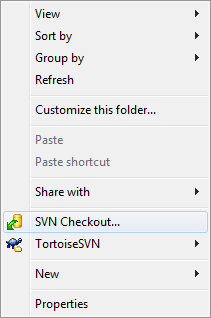
\includegraphics[width=0.40\textwidth]{figures/tortoise_svn_checkout.png}
	\caption{Selecting \textit{SVN Checkout} from the context menu after installing TortoiseSVN.}
	\label{fig:tortoise_svn_checkout}
\end{figure}
\clearpage

A window will now appear that will ask you for the URL of the repository that you would like to access. Our code repository is stored at \url{https://www.cryptool.org/svn/CrypTool2/trunk/}, and this is what you should enter in the appropriate field. The \textit{Checkout directory} should already be filled in correctly with your new folder, and you shouldn't need to change any other options.

\begin{figure}[h!]
	\centering
		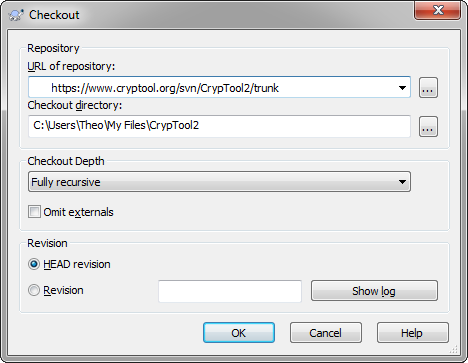
\includegraphics[width=0.60\textwidth]{figures/tortoise_svn_checkout_window.png}
	\caption{Checking out the CrypTool 2 repository.}
	\label{fig:tortoise_svn_checkout2}
\end{figure}

Then just hit \textit{OK}. You may be asked to accept a certificate (which you should accept), and you will certainly be asked for login information. You can use the \textit{anonymous} user with no password for readonly access. If you are a registered developer, you should have already been given a username and password, and you should enter them here. (These are the same username and password that you can use for the \href{https://www.cryptool.org/trac/CrypTool2/wiki}{CrypTool 2 development wiki}.) If you are a guest and just want to download the source code, you can use ``anonymous'' as the username and an empty password. Mark the checkbox for saving your credentials if you don't want to enter them every time you work with the repository (your password will be saved on your computer). Finally, hit \textit{OK}, and the whole CrypTool 2 repository will begin downloading into your chosen local directory.

Since CrypTool 2 is a collaborative project with many developers, changes are made to the repository rather frequently. You should maintain a current working copy of the files to ensure your interoperability with the rest of the project, and thus you should update to the latest version as often as possible. You can do this by right-clicking on any directory within the working files and choosing \textit{SVN~Update} from the context menu.

A TortoiseSVN tutorial can be found at \url{http://www.mind.ilstu.edu/research/robots/iris5/developers/documentation/svntutorial/}.
\clearpage

\subsection{Adjusting the SVN settings}
\label{AdjustingTheSVNSettings}

If you are a registered developer, you can commit your file changes to the public CrypTool 2 repository. However, before you do, you should edit your settings to make sure that you only check in proper source code. First, bring up the TortoiseSVN settings window:

\begin{figure}[h!]
	\centering
		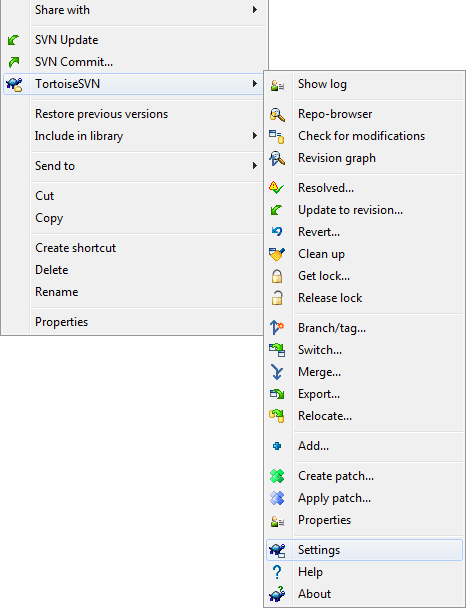
\includegraphics[width=0.70\textwidth]{figures/tortoise_svn_accessing_settings.png}
	\caption{Getting to the TortoiseSVN settings.}
	\label{fig:tortoise_svn_accessing_settings}
\end{figure}
\clearpage

\noindent The settings window will look something like this:

\begin{figure}[h!]
	\centering
		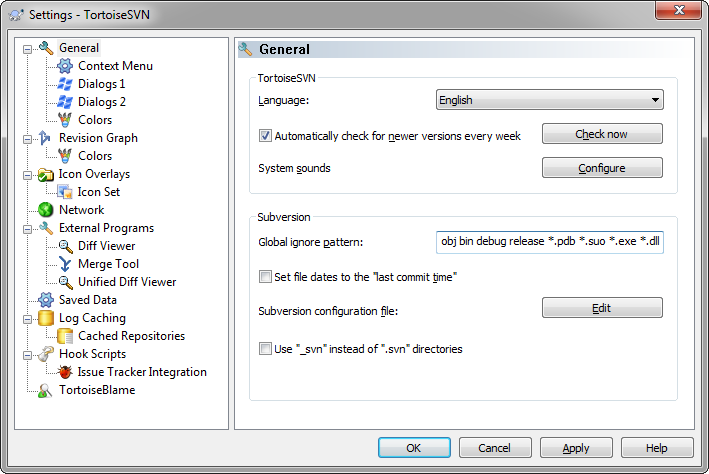
\includegraphics[width=0.90\textwidth]{figures/tortoise_svn_ignore_patterns.png}
	\caption{The TortoiseSVN settings window with the proper ignore pattern.}
	\label{fig:tortoise_svn_ignore_patterns}
\end{figure}

\noindent Then in the \textit{Global ignore pattern} field, please enter the following text:

\begin{center}
\textit{obj bin debug release *.pdb *.suo *.exe *.dll *.aux *.dvi *.log *.bak *.bbl *.blg *.user}
\end{center}

You are free to also leave in any default pattern text or to write your own additions; this pattern serves simply to tell TortoiseSVN what kinds of files to ignore. You can now click \textit{OK} to save your settings and close the window.
\clearpage

\subsection{Committing your changes}
\label{CommitingYourChanges}

Once you start writing code and developing your plugin, you should check your work into the project repository. If you are reading this document in sequence, you are probably not ready to do this, but while we are on the topic of SVN we will describe the process. To upload your changes, right-click on a directory within the working files that contains your changes and select \textit{SVN Commit} from the context menu:

\begin{figure}[h!]
	\centering
		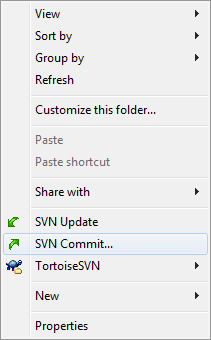
\includegraphics[width=0.40\textwidth]{figures/tortoise_svn_commit.png}
	\caption{Selecting \textit{SVN Commit} from the context menu.}
	\label{fig:tortoise_svn_commit}
\end{figure}
\clearpage

When you commit your code, you must enter a comment to describe what you have changed. \textit{Meaningful descriptions} will help other developers to comprehend your updates. You can also select exactly which files you want to check in. The ignore pattern that we recommended should prevent most undesirable files from being in the list, but double-check to make sure everything you want to upload is included but nothing more. In general, you should never check in compiled and automatically generated files. For example, do not check in the entire \texttt{bin\textbackslash} and \texttt{obj\textbackslash} directories that Visual Studio generates. The server will reject your commits if you try to do so. You should commit your sources to our SVN repository as often as you can, even when it's not finished or when there are bugs. However your committed code should not break anything existing, so please make sure the public solution successfully still compiles and runs.

\begin{figure}[h!]
	\centering
		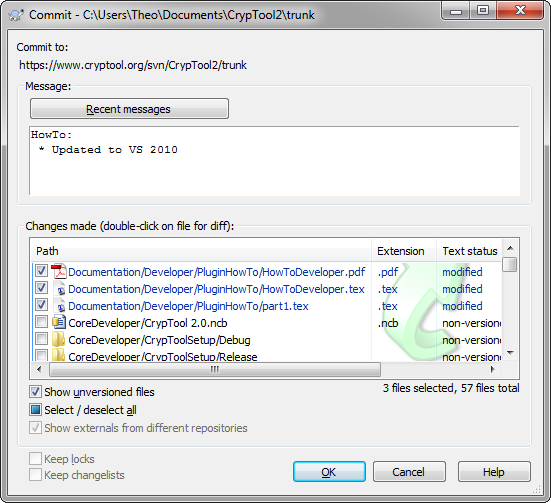
\includegraphics[width=0.70\textwidth]{figures/tortoise_svn_commit_window.png}
	\caption{Providing comments for a commit.}
	\label{fig:tortoise_svn_commit2}
\end{figure}

You can use the SVN comments to link to your changes to a particular issue or bug ticket on the CrypTool 2 development wiki. (The list of active tickets can be found \href{https://www.cryptool.org/trac/CrypTool2/report/1}{here}.) The following commands are supported (note that there are multiple variations of each command that are functionally identical):

\begin{center}
\fbox{\parbox{15cm}
{
\texttt{closes, fixes:}

The specified ticket will be closed and the contents of this commit message will be added to its notes.\\

\texttt{references, refs, addresses, re:}

The contents of this commit message will be added to the specified ticket's notes, but the status will be left unaltered.
}}
\end{center}
\clearpage

You can apply the commands to multiple tickets simultaneously. The command syntax is as follows (again note that there are multiple variations that are functionally identical):

\begin{center}
\fbox{\parbox{15cm}
{\tt
command \#1\\
command \#1, \#2\\
command \#1 \& \#2\\
command \#1 and \#2
}}
\end{center}

You can also use more than one command in a message if necessary. For example, if you want to close tickets \#10 and \#12, and add a note to \#17, you could type the following:

\begin{center}
\fbox{\parbox{15cm}
{\tt
Changed blah and foo to do this or that.\ Fixes \#10 and \#12, and refs \#17.
}}
\end{center}

The comments can also be used to override the ignore pattern that the server is designed to block. However, please do not do this unless you are absolutely sure that you know what you are doing. If you are, you must use the \textit{override-bad-extension} command and provide an explicit list of the file and directory names that you want to upload that need to override the ignore pattern. For example, if you want to check in a library file named \textit{someLib.dll}, you must write something like the following:

\begin{center}
\fbox{\parbox{15cm}
{\tt
This library is referenced by project xy.\\\\
override-bad-extension:\ someLib.dll
}}
\end{center}

Note that any text after the colon and the whitespace will be treated as the file name. Therefore, do not use quotation marks and do not write any text after the file name.

\section{Compiling the sources with Visual Studio 2010}
\label{CompilingTheSourcesVS}

By this point you should have checked out a copy of the entire CrypTool~2 repository. Compiling is pretty easy; just go to the \texttt{trunk\textbackslash} directory and open the \textbf{\textit{CrypTool 2.0.sln}} Visual Studio solution. The Visual Studio IDE should open with all the working plugin components nicely arranged. If you are now starting Visual Studio for the first time, you will have to choose your settings. Just select either \textit{most common} or \textit{C\#} --- you can change this at any time later. On the right side is the project explorer, where you can see all the subprojects included in the solution. Look for the project \textbf{\textit{CrypStartup}} there and make sure it is selected as startup project (right-click on it and select \textit{Set as StartUp Project} from the context menu). Next, go to the menu bar and make sure the target platform is set correctly (Figure~\ref{fig:vs_menubar_x86}). If your operating system is a 32 bit installation, you have to select \textbf{x86}. If you have a 64 bit operating system, you may use one of both, x64 or x86. If in doubt, select x86. Then click \textit{Build $\rightarrow$ Build Solution} in the menubar to start the build process.

\begin{figure}[htbp]
	\centering
		
\includegraphics{figures/vs_menubar_x86.png}
	\caption{Selecting x86 as target platform.}
	\label{fig:vs_menubar_x86}
\end{figure}
\clearpage

You may have to wait a while for the program to compile. Once it is finished, select \textit{Debug $\rightarrow$ Start Debugging}. CrypTool 2 should now start for the first time with your own compiled code. Presumably you have not changed anything yet, but you now have your own build of all the components (with the exception of \textit{CrypWin} and \textit{AnotherEditor}, since they are available only as binaries). If the program does not compile or start correctly, please consult our \href{https://www.cryptool.org/trac/CrypTool2/wiki/FAQ}{FAQ} and let us know if you found a bug.

If you are a \textbf{core developer}, hence somebody who can also compile CrypWin and AnotherEditor, you can use the \textbf{\textit{CrypTool 2.0.sln}} solution from the \texttt{CoreDeveloper\textbackslash} directory (which will \textit{not} be visible to you if you are not a core developer). As a core developer, be aware that when you compile, you \textbf{change the \textit{CrypWin.exe}} that is visible to everybody else. Thus, when committing to the repository, please make sure you \textit{really} want to check in a new binary.

\section{Compiling the sources with Visual C\# 2010 Express}
\label{CompilingTheSourcesExpress}

With Visual C\# Express the build process is basically the same as with Visual Studio. When opening the solution file, you will receive two error messages. The first is because Visual C\# does not support solution folders and shows all plugin projects as a flat list in the solution explorer. However this is only a visual defect. The second error message is, because Visual C\# does not support unit tests and thus is not able to load the project \textit{DevTestMethods}. Again, this does not interfere with opening, writing, compiling, running or debugging plugins.

\section{Downloading the plugin template}
\label{DownloadingThePluginTemplate}

Before you can start implementing a new plugin, you will have to download the CrypTool~2 plugin template. The template is located at the CrypTool 2 website at \url{http://www.cryptool2.vs.uni-due.de/index.php?page=33&lm=3}. Save the template zip file in your documents folder in the subdirectory \texttt{Visual Studio 2010\textbackslash{}Templates\textbackslash{}Project Templates\textbackslash{}} (applies to both, Visual Studio and Visual C\# Express). Do not unpack the zip file.

	\chapter{Plugin Implementation}
\label{sec:PluginImplementation}
In this chapter we provide step-by-step instructions for implementing your own CrypTool 2.0 plugin. The given instructions refer primarily to the usage of the Visual C\# Express and Visual Studio Professional 2008 editions, so before starting you should have a copy of \textbf{Microsoft Visual Studio 2008} (or \textbf{Microsoft Visual C\# 2008 Express Edition}) installed on your computer. We will use the \textbf{Caesar cipher} (also known as the \textbf{shift cipher}) as an example throughout this chapter.

\section{Creating a new project}
\label{sec:CreatingANewProject}

To begin, open Visual Studio, go to the menu bar and select \textit{File~$\rightarrow$ New $\rightarrow$ Project\ldots }. The following window will appear:

\begin{figure}[h!]
	\centering
		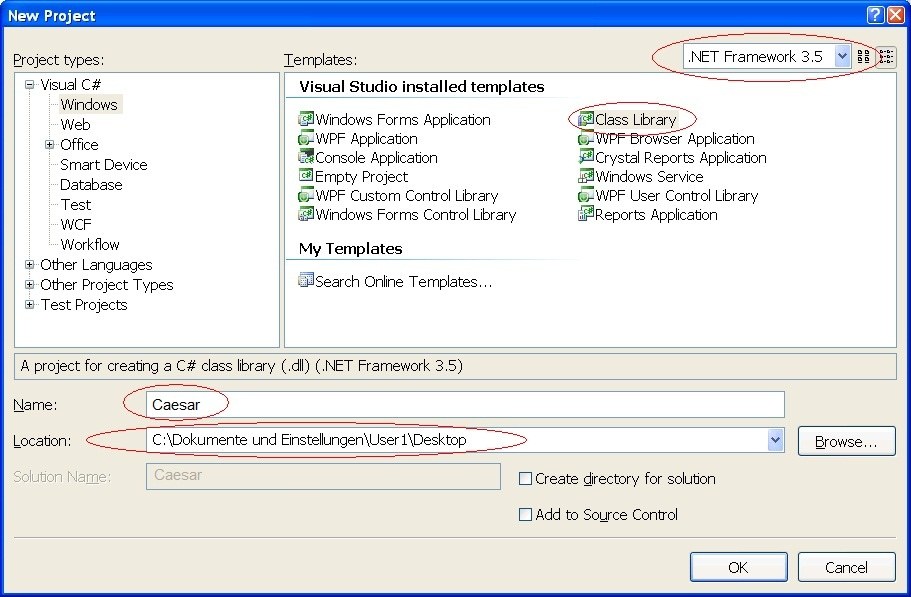
\includegraphics[width=1.00\textwidth]{figures/vs_create_new_project.jpg}
	\caption{Creating a new Visual Studio project.}
	\label{fig:vs_create_new_project}
\end{figure}

\noindent If you are using Visual Studio 2008, select \textbf{\textit{.NET-Framework 3.5}} as the target framework; the Express Edition will automatically choose the target framework. Then choose \textit{Class Library} as the default template, as this will build the project for your plugin as a DLL file. Give the project a unique and meaningful name (such as \textit{Caesar} in our case), and choose a location to save it to. (The Express Edition will ask for a save location later when you close your project or environment). Select the subdirectory \textit{CrypPlugins} from your SVN trunk as the location. Finally, confirm by pressing the \textit{OK} button. Note that creating a new project in this manner also creates a new solution into which the project is placed.

\begin{figure}[h!]
	\centering
		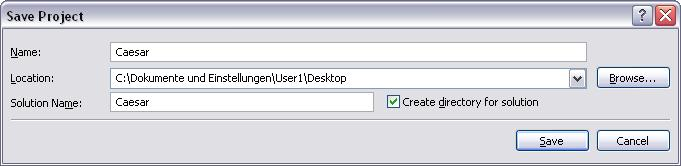
\includegraphics[width=0.80\textwidth]{figures/save_solution_csharp_express.JPG}
	\caption{The Visual Studio C\# Express Edition \textit{Save Project} dialog window.}
	\label{fig:save_solution_csharp_express}
\end{figure}

\noindent At this point, your Visual Studio solution should look like this:

\begin{figure}[h!]
	\centering
		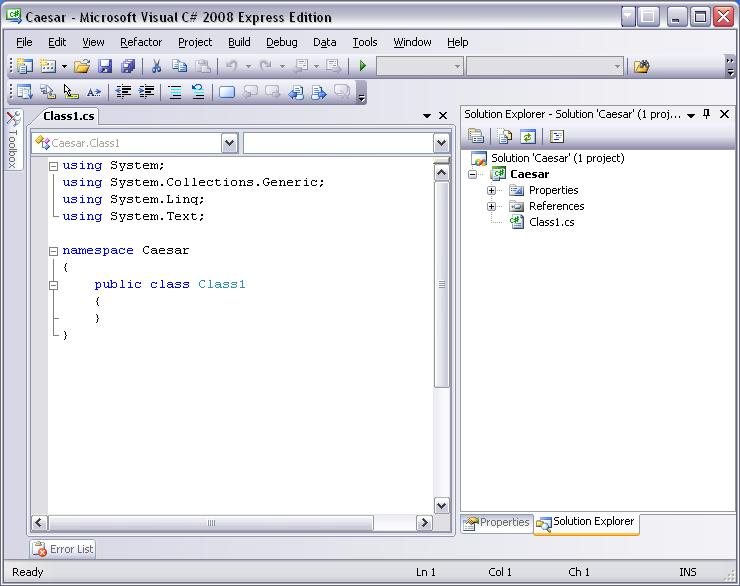
\includegraphics[width=1.00\textwidth]{figures/solution_start_up.jpg}
	\caption{A newly created solution and project.}
	\label{fig:solution_start_up}
\end{figure}
\clearpage

\section{Interface selection}
\label{sec:InterfaceSelection}

To include our new plugin in the CrypTool 2 application, we must first add a reference to the CrypTool 2 library \textbf{\textit{CrypPluginBase.dll}}, where all the necessary CrypTool 2 plugin interfaces are declared.

\begin{figure}[h!]
	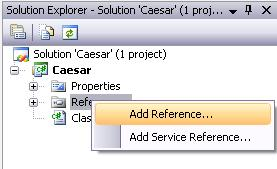
\includegraphics{figures/add_reference.jpg}
	\caption{Adding a new reference.}
	\label{fig:add_reference}
\end{figure}

\noindent Right-click in the Solution Explorer on the \textit{Reference} item and choose \textit{Add Reference}. A window like the following should appear:

\begin{figure}[h!]
	\centering
		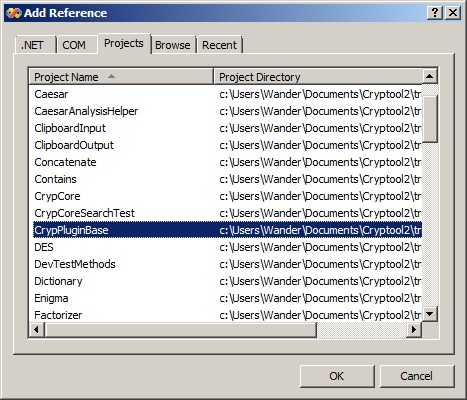
\includegraphics{figures/add_pluginbase_source.jpg}
	\caption{Adding a reference to the CrypPluginBase source code.}
	\label{fig:add_pluginbase_source}
\end{figure}
\clearpage

Unless you have created your new project in the same CrypTool 2.0 solution, you probably will not be able to select the library directly as seen above in Figure \ref{fig:add_pluginbase_source}; instead you can browse for the binary DLL as seen below in Figure \ref{fig:browse_reference}. Click on the \textit{Browse} tab and navigate to the folder in which you downloaded the CrypTool 2 project. Within that folder, go to \textit{\textbackslash CrypPluginBase\textbackslash bin\textbackslash Debug} and select the file \textit{CrypPluginBase.dll}. The library reference can then be added by double clicking the file or pressing the \textit{OK} button.

\begin{figure}[h!]
	\centering
		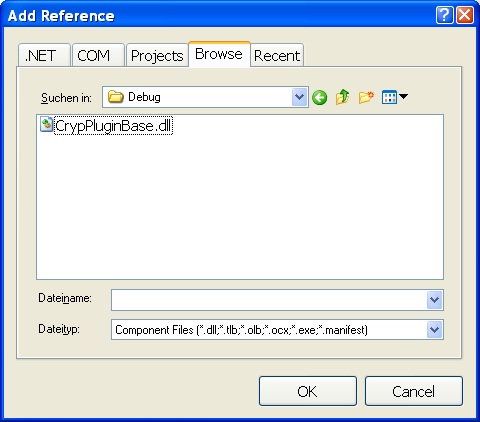
\includegraphics{figures/browse_reference.jpg}
	\caption{Browsing for a reference.}
	\label{fig:browse_reference}
\end{figure}

Besides CrypPluginBase you will need to add three Windows assembly references to provide the necessary namespaces for the user control functions \textit{Presentation} and \textit{QuickWatchPresentation}. This can be done in a similar manner as before with the \textit{CrypPluginBase} reference, but by selecting the \textit{.NET} tab and searching for the references there. Select the following .NET components:

\textit{
\begin{itemize}
    \item PresentationCore
    \item PresentationFramework
    \item WindowsBase
\end{itemize}}
\clearpage

\noindent After these additions, your reference tree view should look like this:

\begin{figure}[h!]
		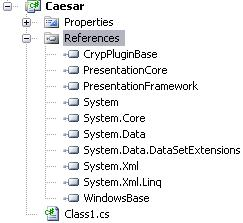
\includegraphics{figures/reference_tree.jpg}
	\caption{A reference tree with the essential components.}
	\label{fig:reference_tree}
\end{figure}

\noindent If your plugin will require other additional libraries, you can add them in the same way.

\section{Modifing the project properties}
\label{sec:ModifyTheProjectProperties}

It is important to make two small changes to your plugin's assembly data to make sure that it will be imported correctly into CrypTool 2. Go to the Solution Explorer and open \textit{AssemblyInfo.cs}, which can be found in the \textit{Properties} folder. Make the following two changes:

\begin{itemize}
	\item Change the attribute \textit{AssemblyVersion} to have the value "2.0.*", and
	\item Comment out the attribute \textit{AssemblyFileVersion}.
\end{itemize}

\noindent This section of your assembly file should now look something like this:

\begin{lstlisting}
[assembly: AssemblyVersion("2.0.*")]
//[assembly: AssemblyFileVersion("1.0.0.0")]
\end{lstlisting}

\section{Creating classes for the algorithm and its settings}
\label{sec:CreatingClassesForTheAlgorithmAndItsSettings}

In the next step we will create two classes. The first class will be the main driver; we will call ours \textit{Caesar} since that is the name of the cipher that it will implement. In our case, this class has to inherit from \textit{IEncryption} because it will be an encryption plugin. If it was instead a hash plugin, this class should inherit from \textit{IHash}. The second class will be used to store setting information for the plugin, and thus we will name ours \textit{CaesarSettings}. It will need to inherit from \textit{ISettings}.
\clearpage

\subsection{Creating a class for the algorithm}
\label{sec:CreatingAClassForTheAlgorithm}

When starting a new project, Visual Studio automatically creates a class named \textit{Class1.cs}. Since this is a rather non-descriptive name, we will change it. In our example, it will be \textit{Caesar.cs}. There are two ways to change the name:

\begin{itemize}
	\item Rename the existing class, or
	\item Delete the existing class and create a new one.
\end{itemize}
%\clearpage

\noindent Both options will achieve the same results. We will guide you through the second method. First, delete \textit{Class1.cs}.

\begin{figure}[h!]
	\centering
		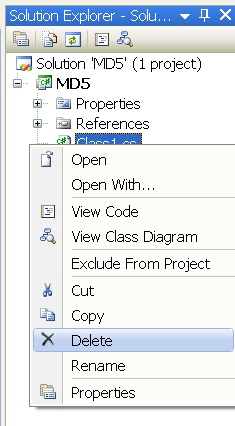
\includegraphics{figures/new_class.jpg}
	\caption{Deleting a class.}
	\label{fig:new_class}
\end{figure}
\clearpage

\noindent Then right-click on the project item (in our case, \textit{Caesar}) and select \textit{Add $\rightarrow$ Class\ldots }:

\begin{figure}[h]
	\centering
		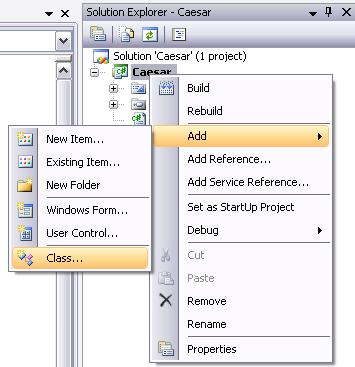
\includegraphics{figures/add_new_class.jpg}
	\caption{Adding a new class.}
	\label{fig:add_new_class}
\end{figure}
\clearpage

\noindent Finally, give your class a unique name. We will call our class \textit{Caesar.cs} and define it as public so that it will be available to other classes.

\begin{figure}[h!]
	\centering
		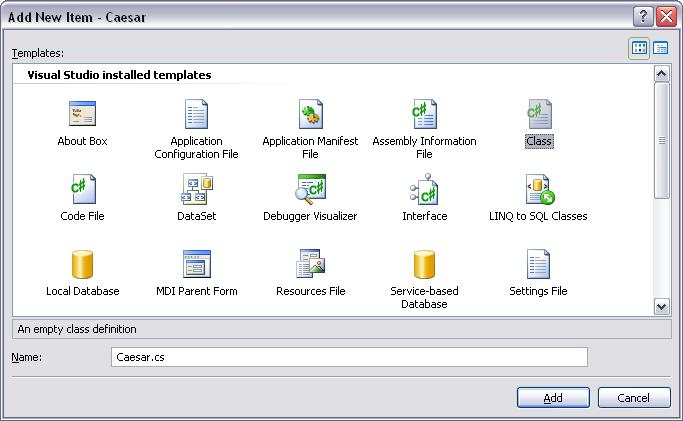
\includegraphics[width=1.00\textwidth]{figures/name_new_class.jpg}
	\caption{Naming the new class.}
	\label{fig:name_new_class}
\end{figure}

Note that Visual Studio will automatically generate a very basic code outline for the new class. In our example, we will not use the all the namespaces that are automatically imported, so you can delete the lines \texttt{using System;} and \texttt{using System.Linq;}.

\subsection{Creating a settings class}
\label{sec:CreatingASettingsClass}

Add a second public class in the same way. We will call the class \textit{CaesarSettings}. The settings class will store the necessary information about controls, captions, descriptions and default parameters (e.g.\ for key settings, alphabets, key length and type of action) to build the \textbf{TaskPane} in the CrypTool application.
\clearpage

\noindent Below is an example of what a completed TaskPane for the existing Caesar plugin in CrypTool 2 looks like:

\begin{figure}[h!]
	\centering
		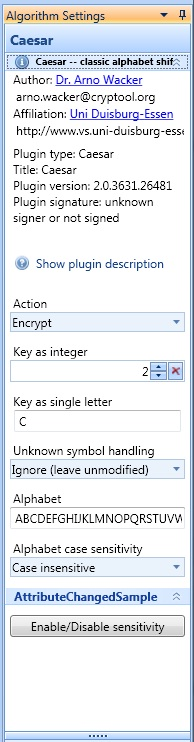
\includegraphics{figures/task_pane.jpg}
	\caption{The completed TaskPane for the existing Caesar plugin.}
	\label{fig:task_pane}
\end{figure}
\clearpage

\subsection{Adding the namespaces and inheritance sources for the Caesar class}
\label{sec:AddingTheNamespacesAndInheritanceSourcesForTheCaesarClass}

Open the \textit{Caesar.cs} file by double clicking on it in the Solution Explorer. To include the necessary namespaces in the class header, use the \texttt{using} statement followed by the name of the desired namespace. The CrypTool 2 API provides the following namespaces:

\begin{itemize}
	\item \textit{Cryptool.PluginBase} --- contains interfaces such as \textit{IPlugin}, \textit{IHash}, and \textit{ISettings}, as well as attributes, enumerations, delegates and extensions.
	\item \textit{Cryptool.PluginBase.Analysis} --- contains interfaces for cryptanalysis plugins (such as \textit{Stream Comparator}).
	\item \textit{Cryptool.PluginBase.Control} --- contains global interfaces for the \textit{IControl} feature for defining custom controls.
	\item \textit{Cryptool.PluginBase.Cryptography} --- contains interfaces for encryption and hash algorithms such as AES, DES and MD5.
	\item \textit{Cryptool.PluginBase.Editor} --- contains interfaces for editors that can be implemented in CrypTool 2, such as the default editor.
	\item \textit{Cryptool.PluginBase.Generator} --- contains interfaces for generators, including the random input generator.
	\item \textit{Cryptool.PluginBase.IO} --- contains interfaces for input, output and the \textit{CryptoolStream}.
	\item \textit{Cryptool.PluginBase.Miscellaneous} --- contains assorted helper classes, including \textit{GuiLogMessage} and \textit{PropertyChanged}.
	\item \textit{Cryptool.PluginBase.Resources} --- used only by CrypWin and the editor; not necessary for plugin development.
	\item \textit{Cryptool.PluginBase.Tool} --- contains an interface for all external tools implemented by CrypTool~2 that do not entirely support the CrypTool 2 API.
	\item \textit{Cryptool.PluginBase.Validation} --- contains interfaces for validation methods, including regular expressions.
\end{itemize}

\noindent In our example, the Caesar algorithm necessitates the inclusion of the following namespaces:

\begin{itemize}
	\item \textit{Cryptool.PluginBase} --- to implement \textit{ISettings} in the CaesarSettings class.
	\item \textit{Cryptool.PluginBase.Cryptography} --- to implement \textit{IEncryption} in the Caesar class.
	\item \textit{Cryptool.PluginBase.IO} --- to use CryptoolStream for data input and output.
	\item \textit{Cryptool.PluginBase.Miscellaneous} --- to use the CrypTool event handler.
\end{itemize}

\noindent It is important to define a new default namespace for our public class (\textit{Caesar}). In CrypTool 2  the standard namespace convention is \textit{Cryptool.[name of class]}. Therefore our namespace will be defined as \textit{Cryptool.Caesar}.\clearpage

\noindent At this point, the source code should look like the following:

\begin{lstlisting}
using System.Collections.Generic;
using System.Text;

//required CrypTool namespaces
using Cryptool.PluginBase;
using Cryptool.PluginBase.Cryptography;
using Cryptool.PluginBase.IO;
using Cryptool.PluginBase.Miscellaneous;

namespace Cryptool.Caesar
{
	public class Caesar
	{
	}
}
\end{lstlisting}

\ \\ % ugly but functional
\noindent Next we should let the \textit{Caesar} class inherit from \textit{IEncryption} by making the following alteration:

\begin{lstlisting}
namespace Cryptool.Caesar
{
	public class Caesar : IEncryption
	{
	}
}
\end{lstlisting}

\subsection{Adding interface functions to the Caesar class}
\label{sec:AddingInterfaceFunctionsToTheCaesarClass}

You may notice an underscore underneath the ``I'' in ``IEncryption''. Move your mouse over it, or place the cursor on it and press ``Shift+Alt+F10'' and the following submenu should appear:

\begin{figure}[h!]
	\centering
		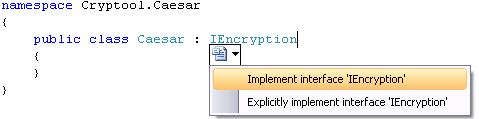
\includegraphics{figures/inherit_submenu.jpg}
	\caption{An inheritance submenu.}
	\label{fig:inherit_submenu}
\end{figure}

Select the item ``Implement interface `IEncryption'\,''. Visual Studio will automatically generate all the interface members necessary for interaction with the CrypTool 2 core. (This step will save you a lot of typing!)
\clearpage

\noindent Your code should now look like this:

\begin{lstlisting}
using System.Collections.Generic;
using System.Text;

using Cryptool.PluginBase;
using Cryptool.PluginBase.Cryptography;
using Cryptool.PluginBase.IO;
using Cryptool.PluginBase.Miscellaneous;

namespace Cryptool.Caesar
{
    public class Caesar : IEncryption
    {
        #region IPlugin Members

        public void Dispose()
        {
            throw new NotImplementedException();
        }

        public void Execute()
        {
            throw new NotImplementedException();
        }

        public void Initialize()
        {
            throw new NotImplementedException();
        }

        public event GuiLogNotificationEventHandler OnGuiLogNotificationOccured;

        public event PluginProgressChangedEventHandler OnPluginProgressChanged;

        public event StatusChangedEventHandler OnPluginStatusChanged;

        public void Pause()
        {
            throw new NotImplementedException();
        }

        public void PostExecution()
        {
            throw new NotImplementedException();
        }

        public void PreExecution()
        {
            throw new NotImplementedException();
        }

        public System.Windows.Controls.UserControl Presentation
        {
            get { throw new NotImplementedException(); }
        }

        public System.Windows.Controls.UserControl QuickWatchPresentation
        {
            get { throw new NotImplementedException(); }
        }

        public ISettings Settings
        {
            get { throw new NotImplementedException(); }
        }

        public void Stop()
        {
            throw new NotImplementedException();
        }

        #endregion

        #region INotifyPropertyChanged Members

        public event System.ComponentModel.PropertyChangedEventHandler PropertyChanged;

        #endregion
    }
}
\end{lstlisting}

\subsection{Adding the namespace and interfaces to the CaesarSettings class}
\label{sec:AddingTheNamespaceAndInterfacesToTheCaesarSettingsClass}

Let's now take a look at the second class in our example, ``CaesarSettings'', by double-clicking on the ``CaesarSettings.cs'' file in the Solution Explorer. First, we need to again include the ``Cryptool.PluginBase'' namespace to the class header. Then we must let the settings class inherit from ``ISettings'' in the same manner as was done with the Caesar class. Visual Studio will again automatically generate code from the CrypTool interface as seen below. (We can again remove the lines \texttt{using System;} and \texttt{using System.Linq;}, as we do not need those references.)\\

\begin{lstlisting}
using System.Collections.Generic;
using System.Text;

using Cryptool.PluginBase;

namespace Cryptool.Caesar
{
    public class CaesarSettings : ISettings
    {
        #region ISettings Members

        public bool HasChanges
        {
            get
            {
                throw new NotImplementedException();
            }
            set
            {
                throw new NotImplementedException();
            }
        }

        #endregion

        #region INotifyPropertyChanged Members

        public event System.ComponentModel.PropertyChangedEventHandler PropertyChanged;

        #endregion
    }
}
\end{lstlisting}

\subsection{Adding controls to the CaesarSettings class}
\label{sec:AddingControlsToTheCaesarSettingsClass}

The settings class is used to populate the TaskPane in the CrypTool 2 application so that the user can modify settings at will. To meet these ends we will need to implement some controls such as buttons and text boxes. If you will be implementing an algorithm that does not have any user-defined settings (i.e.\ a hash function), then this class can be left empty; you will, however, still have to modify the ``HasChanges'' property to avoid a ``NotImplementedException''. The following code demonstrates the modifications necessary to create the backend for the TaskPane for our Caesar algorithm. You can also look at the source code of other algorithms in the subversion repository for examples of how to create the TaskPane backend.\\

\begin{lstlisting}
using System;
using System.ComponentModel;
using System.Windows;
using Cryptool.PluginBase;
using System.Windows.Controls;

namespace Cryptool.Caesar
{
    public class CaesarSettings : ISettings
    {
        #region Public Caesar specific interface

        /// <summary>
        /// We use this delegate to send log messages from
        /// the settings class to the Caesar plugin.
        /// </summary>
        public delegate void CaesarLogMessage(string msg, NotificationLevel loglevel);

        /// <summary>
        /// An enumeration for the different modes of handling
        /// unknown characters.
        /// </summary>
        public enum UnknownSymbolHandlingMode { Ignore = 0, Remove = 1, Replace = 2 };

        /// <summary>
        /// Fires when a new status message was sent.
        /// </summary>
        public event CaesarLogMessage LogMessage;

        public delegate void CaesarReExecute();

        public event CaesarReExecute ReExecute;

        /// <summary>
        /// Retrieves or sets the current shift value (i.e. the key).
        /// </summary>
        [PropertySaveOrder(0)]
        public int ShiftKey
        {
            get { return shiftValue; }
            set
            {
                setKeyByValue(value);
            }
        }

        /// <summary>
        /// Retrieves the current setting of whether or not the
        /// alphabet should be treated as case-sensitive.
        /// </summary>
        [PropertySaveOrder(1)]
        public bool CaseSensitiveAlphabet
        {
            get
            {
                if (caseSensitiveAlphabet == 0)
                {   return false;   }
                else
                {   return true;    }
            }
            set {} // this setting is readonly, but we must include
                   // some form of set method to prevent problems.
        }


        /// <summary>
        /// Returns true if any settings have been changed.
        /// This value should be set externally to false, i.e.
        /// when a project is saved.
        /// </summary>
        [PropertySaveOrder(3)]
        public bool HasChanges
        {
            get { return hasChanges; }
            set { hasChanges = value; }
        }

        #endregion

        #region Private variables
        private bool hasChanges;
        private int selectedAction = 0;
        private string upperAlphabet = "ABCDEFGHIJKLMNOPQRSTUVWXYZ";
        private string lowerAlphabet = "abcdefghijklmnopqrstuvwxyz";
        private string alphabet = "ABCDEFGHIJKLMNOPQRSTUVWXYZ";
        private char shiftChar = 'C';
        private int shiftValue = 2;
        private UnknownSymbolHandlingMode unknownSymbolHandling = UnknownSymbolHandlingMode.Ignore;
        private int caseSensitiveAlphabet = 0; // 0 = case-insensitve, 1 = case-sensitive
        private bool sensitivityEnabled = true;
        #endregion

        #region Private methods

        private string removeEqualChars(string value)
        {
            int length = value.Length;

            for (int i = 0; i < length; i++)
            {
                for (int j = i + 1; j < length; j++)
                {
                    if ((value[i] == value[j]) || (!CaseSensitiveAlphabet & (char.ToUpper(value[i]) == char.ToUpper(value[j]))))
                    {
                        LogMessage("Removing duplicate letter: \'" + value[j] + "\' from alphabet!", NotificationLevel.Warning);
                        value = value.Remove(j,1);
                        j--;
                        length--;
                    }
                }
            }

            return value;
        }

        /// <summary>
        /// Set the new shiftValue and the new shiftCharacter
        /// to offset % alphabet.Length.
        /// </summary>
        private void setKeyByValue(int offset)
        {
            HasChanges = true;

            // Make sure the shift value lies within the alphabet range.
            offset = offset % alphabet.Length;

            // Set the new shiftChar.
            shiftChar = alphabet[offset];

            // Set the new shiftValue.
            shiftValue = offset;

            // Announce this to the settings pane.
            OnPropertyChanged("ShiftValue");
            OnPropertyChanged("ShiftChar");

            // Print some info in the log.
            LogMessage("Accepted new shift value " + offset + "! (Adjusted shift character to \'" + shiftChar + "\')", NotificationLevel.Info);
        }

        private void setKeyByCharacter(string value)
        {
            try
            {
                int offset;
                if (this.CaseSensitiveAlphabet)
                {
                    offset = alphabet.IndexOf(value[0]);
                }
                else
                {
                    offset = alphabet.ToUpper().IndexOf(char.ToUpper(value[0]));
                }

                if (offset >= 0)
                {
                    HasChanges = true;
                    shiftValue = offset;
                    shiftChar = alphabet[shiftValue];
                    LogMessage("Accepted new shift character \'" + shiftChar + "\'! (Adjusted shift value to " + shiftValue + ")", NotificationLevel.Info);
                    OnPropertyChanged("ShiftValue");
                    OnPropertyChanged("ShiftChar");
                }
                else
                {
                    LogMessage("Bad input \"" + value + "\"! (Character not in alphabet!) Reverting to " + shiftChar.ToString() + "!", NotificationLevel.Error);
                }
            }
            catch (Exception e)
            {
                LogMessage("Bad input \"" + value + "\"! (" + e.Message + ") Reverting to " + shiftChar.ToString() + "!", NotificationLevel.Error);
            }
        }

        #endregion

        #region Algorithm settings properties (visible in the Settings pane)

        [PropertySaveOrder(4)]
        [ContextMenu("Action", "Select the algorithm action", 1, DisplayLevel.Beginner, ContextMenuControlType.ComboBox, new int[] { 1, 2 }, "Encrypt", "Decrypt")]
        [TaskPane("Action", "setAlgorithmActionDescription", null, 1, true, DisplayLevel.Beginner, ControlType.ComboBox, new string[] { "Encrypt", "Decrypt" })]
        public int Action
        {
            get
            {
                return this.selectedAction;
            }
            set
            {
                if (value != selectedAction) HasChanges = true;
                this.selectedAction = value;
                OnPropertyChanged("Action");

                if (ReExecute != null) ReExecute();
            }
        }

        [PropertySaveOrder(5)]
        [TaskPane("Key as integer", "Enter the number of letters to shift. For example, a value of 1 means that the plaintext character 'a' gets mapped to the ciphertext character 'B', 'b' to 'C', and so on.", null, 2, true, DisplayLevel.Beginner, ControlType.NumericUpDown, ValidationType.RangeInteger, 0, 100)]
        public int ShiftValue
        {
            get { return shiftValue; }
            set
            {
                setKeyByValue(value);
                if (ReExecute != null) ReExecute();
            }
        }

        [PropertySaveOrder(6)]
        [TaskPaneAttribute("Key as single letter", "Enter a single letter as the key. This letter is mapped to an integer stating the position in the alphabet. The values for 'Key as integer' and 'Key as single letter' are always synchronized.", null, 3, true, DisplayLevel.Beginner, ControlType.TextBox, ValidationType.RegEx, "^([A-Z]|[a-z]){1,1}")]
        public string ShiftChar
        {
            get { return this.shiftChar.ToString(); }
            set
            {
                setKeyByCharacter(value);
                if (ReExecute != null) ReExecute();
            }
        }

        [PropertySaveOrder(7)]
        [ContextMenu("Unknown symbol handling", "What should be done with characters encountered in the input which are not in the alphabet?", 4, DisplayLevel.Expert, ContextMenuControlType.ComboBox, null, new string[] { "Ignore (leave unmodified)", "Remove", "Replace with \'?\'" })]
        [TaskPane("Unknown symbol handling", "What should be done with characters encountered in the input which are not in the alphabet?", null, 4, true, DisplayLevel.Expert, ControlType.ComboBox, new string[] { "Ignore (leave unmodified)", "Remove", "Replace with \'?\'" })]
        public int UnknownSymbolHandling
        {
            get { return (int)this.unknownSymbolHandling; }
            set
            {
                if ((UnknownSymbolHandlingMode)value != unknownSymbolHandling) HasChanges = true;
                this.unknownSymbolHandling = (UnknownSymbolHandlingMode)value;
                OnPropertyChanged("UnknownSymbolHandling");

                if (ReExecute != null) ReExecute();
            }
        }

        [SettingsFormat(0, "Normal", "Normal", "Black", "White", Orientation.Vertical)]
        [PropertySaveOrder(9)]
        [TaskPane("Alphabet", "This is the alphabet currently in use.", null, 6, true, DisplayLevel.Expert, ControlType.TextBox, "")]
        public string AlphabetSymbols
        {
          get { return this.alphabet; }
          set
          {
            string a = removeEqualChars(value);
            if (a.Length == 0) // cannot accept empty alphabets
            {
              LogMessage("Ignoring empty alphabet from user! Using previous alphabet instead: \" + alphabet + "\" (" + alphabet.Length.ToString() + " Symbols)", NotificationLevel.Info);
            }
            else if (!alphabet.Equals(a))
            {
              HasChanges = true;
              this.alphabet = a;
              setKeyByValue(shiftValue); // reevaluate if the shiftvalue is still within the range
              LogMessage("Accepted new alphabet from user: \" + alphabet + "\" (" + alphabet.Length.ToString() + " Symbols)", NotificationLevel.Info);
              OnPropertyChanged("AlphabetSymbols");

              if (ReExecute != null) ReExecute();
            }
          }
        }

        /// <summary>
        /// Visible setting how to deal with alphabet case.
        /// 0 = case-insentive, 1 = case-sensitive
        /// </summary>
        //[SettingsFormat(1, "Normal")]
        [PropertySaveOrder(8)]
        [ContextMenu("Alphabet case sensitivity", "Should upper and lower case be treated as the same (so that 'a' = 'A')?", 7, DisplayLevel.Expert, ContextMenuControlType.ComboBox, null, new string[] { "Case insensitive", "Case sensitive" })]
        [TaskPane("Alphabet case sensitivity", "Should upper and lower case be treated as the same (so that 'a' = 'A')?", null, 7, true, DisplayLevel.Expert, ControlType.ComboBox, new string[] { "Case insensitive", "Case sensitive" })]
        public int AlphabetCase
        {
            get { return this.caseSensitiveAlphabet; }
            set
            {
                if (value != caseSensitiveAlphabet) HasChanges = true;
                this.caseSensitiveAlphabet = value;
                if (value == 0)
                {
                    if (alphabet == (upperAlphabet + lowerAlphabet))
                    {
                        alphabet = upperAlphabet;
                        LogMessage("Changing alphabet to: \"" + alphabet + "\" (" + alphabet.Length.ToString() + " Symbols)", NotificationLevel.Info);
                        OnPropertyChanged("AlphabetSymbols");
                        // reset the key (shiftvalue/shiftChar)
                        // to be in the range of the new alphabet.
                        setKeyByValue(shiftValue);
                    }
                }
                else
                {
                    if (alphabet == upperAlphabet)
                    {
                        alphabet = upperAlphabet + lowerAlphabet;
                        LogMessage("Changing alphabet to: \"" + alphabet + "\" (" + alphabet.Length.ToString() + " Symbols)", NotificationLevel.Info);
                        OnPropertyChanged("AlphabetSymbols");
                    }
                }

                // Remove equal characters from the current alphabet.
                string a = alphabet;
                alphabet = removeEqualChars(alphabet);
                if (a != alphabet)
                {
                    OnPropertyChanged("AlphabetSymbols");
                    LogMessage("Changing alphabet to: \"" + alphabet + "\" (" + alphabet.Length.ToString() + " Symbols)", NotificationLevel.Info);
                }
                OnPropertyChanged("AlphabetCase");
                if (ReExecute != null) ReExecute();
            }
        }

        #endregion

        #region INotifyPropertyChanged Members

        public event PropertyChangedEventHandler PropertyChanged;

        protected void OnPropertyChanged(string name)
        {
          if (PropertyChanged != null)
          {
            PropertyChanged(this, new PropertyChangedEventArgs(name));
          }
        }

        #endregion

        #region TaskPaneAttributeChanged (Sample)
        /// <summary>
        /// This event is here merely as a sample.
        /// </summary>
        public event TaskPaneAttributeChangedHandler TaskPaneAttributeChanged;

        [TaskPane("Enable/Disable sensitivity", "This setting is just a sample and shows how to enable / disable a setting.", "AttributeChangedSample", 8, false, DisplayLevel.Beginner, ControlType.Button)]
        public void EnableDisableSesitivity()
        {
          if (TaskPaneAttributeChanged!= null)
          {
            sensitivityEnabled = !sensitivityEnabled;
            if (sensitivityEnabled)
            {
              TaskPaneAttributeChanged(this, new TaskPaneAttributeChangedEventArgs(new TaskPaneAttribteContainer("AlphabetCase", Visibility.Visible)));
            }
            else
            {
              TaskPaneAttributeChanged(this, new TaskPaneAttributeChangedEventArgs(new TaskPaneAttribteContainer("AlphabetCase", Visibility.Collapsed)));
            }
          }
        }
        #endregion TaskPaneAttributeChanged (Sample)
    }
}
\end{lstlisting}
\clearpage

\section{Adding an icon to the Caesar class}
\label{sec:AddingAnIconToTheCaesarClass}

Before we go back to the code of the Caesar class, we have to add an icon to our project, which will be shown in the CrypTool \textbf{ribbon bar} and \textbf{navigation pane}. As there is currently no default, it is mandatory to add an icon. (It is planned to include a default icon in future versions.)

For testing purposes you can just create a simple black and white PNG image with MS Paint or Paint.NET. The proper image size is 40x40 pixels, but since the image will be rescaled if necessary, any size is technically acceptable.

Once you have saved your icon, you should add it directly to the project or to a subdirectory. In the project solution, we created a new folder named ``Images''. This can be done by right-clicking on the project item (``Caesar'' in our example) and selecting ``Add $\rightarrow$ New Folder''. The icon can be added to this folder (or to the project directly, or to any other subdirectory) by right-clicking on the folder and selecting ``Add $\rightarrow$ Existing Item''.

\begin{figure}[h!]
	\centering
		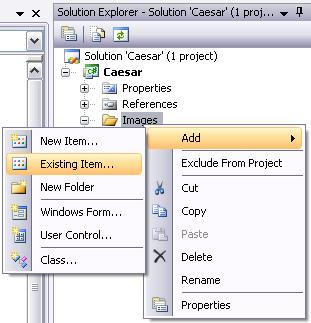
\includegraphics{figures/add_existing_item.jpg}
	\caption{Adding an existing item.}
	\label{fig:add_existing_item}
\end{figure}
\clearpage

A new window will then appear. Select ``Image Files'' as the file type and select your newly-created icon for your plugin.

\begin{figure}[h!]
	\centering
		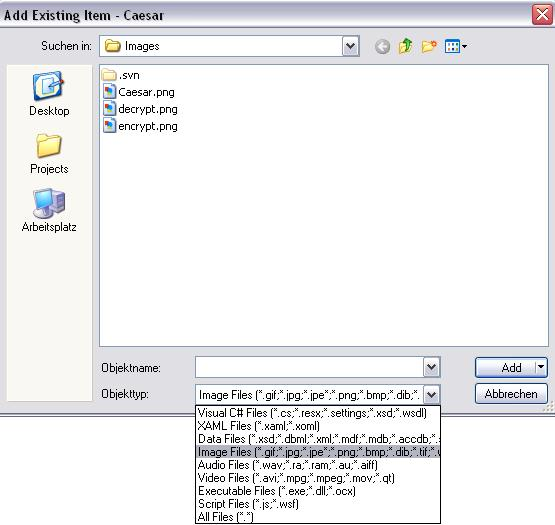
\includegraphics{figures/choose_icon.jpg}
	\caption{Selecting the image file.}
	\label{fig:choose_icon}
\end{figure}
\clearpage

Finally, we must set the icon as a ``Resource'' to avoid including the icon as a separate file. Right-click on the icon and select ``Properties'' as seen below.

\begin{figure}[h!]
	\centering
		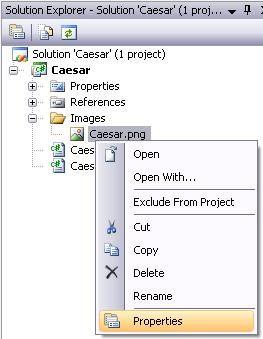
\includegraphics{figures/icon_properties.jpg}
	\caption{Selecting the image properties.}
	\label{fig:icon_properties}
\end{figure}

In the ``Properties'' panel, set the ``Build Action'' to ``Resource''.

\begin{figure}[h!]
	\centering
		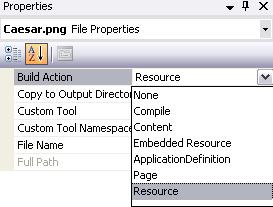
\includegraphics{figures/icon_build_action.jpg}
	\caption{Selecting the icon's build action.}
	\label{fig:icon_build_action}
\end{figure}
\clearpage

\section{Defining the attributes of the Caesar class}
\label{sec:DefiningTheAttributesOfTheCaesarClass}

Now let's go back to the code of the Caesar class (the ``Caesar.cs'' file in our example). The first thing we will do is define the attributes of our class. These attributes are used to provide additional information for the CrypTool 2.0 environment. If they are not properly defined, your plugin won't show up in the application display, even if everything else is implemented correctly.

Attributes are used for \textbf{declarative} programming and provide metadata that can be added to the existing .NET metadata. CrypTool provides a set of custom attributes that are used to mark the different parts of your plugin.

These attributes can be defined anywhere within the ``Cryptool.Caesar'' namespace, but customarily they are defined right before the class declaration.

\subsection{The \protect\textit{[Author]} attribute}
\label{sec:TheAuthorAttribute}

The \textit{[Author]} attribute is optional, and thus we are not required to define it. The attribute can be used to provide additional information about the plugin developer. This information will appear in the TaskPane, as for example in Figure \ref{fig:task_pane}. We will define the attribute to demonstrate how it should look in case you want to use it in your plugin.

\begin{figure}[h!]
	\centering
		
\includegraphics[width=.90\textwidth]{figures/attribute_author_new.jpg}
	\caption{The defintion for the \textit{[Author]} attribute.}
	\label{fig:attribute_author}
\end{figure}

As can be seen above, the author attribute takes four elements of type string. These elements are:

\begin{itemize}
	\item Author --- the name of the plugin developer(s).
	\item Email --- the email address of the plugin developer(s), should they wish to be available for contact.
	\item Institute --- the organization, company or university with which the developer(s) are affiliated.
	\item URL --- the website of the developer(s) or their institution.
\end{itemize}

All of these elements are optional; the developer(s) can choose what information will be published. Unused elements should be set to null or an empty string.
\clearpage

%Our author attribute should look now as you can see below:
%\begin{figure}[h!]
%	\centering
%		
\includegraphics[width=1.00\textwidth]{figures/attribute_author_filled.jpg}
%	\caption{Filled author auttribute}
%	\label{fig:attribute_author_filled}
%\end{figure}

\subsection{The \protect\textit{[PluginInfo]} attribute}
\label{sec:ThePluginInfoAttribute}

The second attribute, \textit{[PluginInfo]}, provides necessary information about the plugin, and is therefore mandatory. This information appears in the caption and tool tip window. The attribute is defined as follows:

\begin{figure}[h]
	\centering
		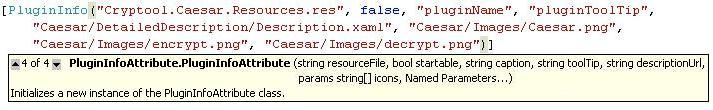
\includegraphics[width=1.00\textwidth]{figures/attribute_plugininfo_new.jpg}
	\caption{The defintion for the \textit{[PluginInfo]} attribute.}
	\label{fig:attribute_plugininfo}
\end{figure}

\noindent This attribute has the following parameters:

\begin{itemize}
	\item Resource File --- defines where to find the associated resource file, if one is to be implemented. These are used, for example, to provide multilingual support for the plugin. This element is optional.
	\item Startable --- a flag that should be set to true only if the plugin is an input generator plugin (i.e.\ if your plugin only has outputs and no inputs). In all other cases this should be set to false. This flag is important --- setting it incorrectly will result in unpredictable results. This element is mandatory.
	\item Caption --- the name of the plugin or, if the caption is specified in a resource file, the name of the appropriate field in the resource file. This element is mandatory.
	\item ToolTip --- a description of the plugin or, if the tool tip is specified in a resource file, the name of the appropriate field in the resource file. This element is optional.
	\item DescriptionURL --- defines where to find the description file (e.g.\ XAML file). This element is optional.
	\item Icons --- an array of strings to define all the paths for the icons to be used in the plugin (i.e.\ the plugin icon described in Section \ref{sec:AddingAnIconToTheCaesarClass}). This element is mandatory.
\end{itemize}

\noindent Unused elements should be set to null or an empty string.

(There are a few limitations and bugs that still exist in the \textit{[PluginInfo]} attribute that will be resolved in a future version. Firstly, it is possible to use the plugin without setting a caption, although this is not recommended. In the future the plugin will fail to load without a caption. Secondly, a zero-length toolTip string currently causes the toolTip to appear as an empty box in the application. Lastly, the toolTip and description do not currently support internationalization and localization.)

In our example, the ``resourceFile'' parameter should be set to ``Cryptool.Caesar.Resource.res''. This file will be used to store the label and caption text to support multilingualism.

%\begin{figure}[h]
%	\centering
%		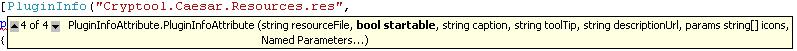
\includegraphics[width=1.00\textwidth]{figures/attribute_plugininfo_resourceFile.JPG}
%	\caption{Attribute PluginInfo element resourceFile}
%	\label{fig:attribute_plugininfo_resourceFile}
%\end{figure}

The second parameter, ``startable'' should be set to ``false'', because our encryption algorithm is not an input generator plugin.

%\begin{figure}[h!]
%	\centering
%		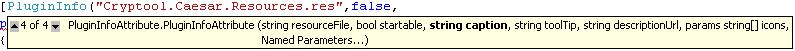
\includegraphics[width=1.00\textwidth]{figures/attribute_plugininfo_startable.jpg}
%	\caption{Attribute PluginInfo startable}
%	\label{fig:attribute_plugininfo_startable}
%\end{figure}

The next two parameters are necessary to define the plugin's name and description. Since we are using a resource file, we should place here the names of the resource fields that contain the description and caption.  (We call also just write simple text strings instead of using outsourced references.)

%\begin{figure}[h!]
%	\centering
%		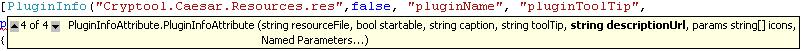
\includegraphics[width=1.00\textwidth]{figures/attribute_plugininfo_description.jpg}
%	\caption{Attribute PluginInfo name and description}
%	\label{fig:attribute_plugininfo_description}
%\end{figure}

The next element defines the location path of the description file. The parameter is composed in the format \textit{$<$assembly name$>$/$<$file name$>$} or, if you want to store your description files in a separate folder (as in our case), \textit{$<$assembly name$>$/$<$path$>$/$<$file name$>$}. The description file must be an XAML file. In our case, we shall create a folder named ``DetailedDescription'' in which to store our XAML file with any necessary images. Our folder structure looks as follows:

\begin{figure}[h!]
	\centering
		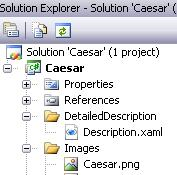
\includegraphics[width=.30\textwidth]{figures/attribute_plugininfo_detailed_descr_path.jpg}
	\caption{The folder structure as seen in the Solution Explorer.}
	\label{fig:attribute_plugininfo_icon_path}
\end{figure}

%Accordingly the attribute parameter has to be set to:
%\begin{figure}[h!]
%	\centering
%		
\includegraphics[width=1.00\textwidth]{figures/attribute_plugininfo_detailed_descr.jpg}
%	\caption{Attribute PluginInfo description file}
%	\label{fig:attribute_plugininfo_icon}
%\end{figure}

Once a detailed description has been written in the XAML file, it can be accessed in the CrypTool 2 application by right-clicking on the plugin icon in the workspace and selecting ``Show description''.

\begin{figure}[h!]
	\centering
		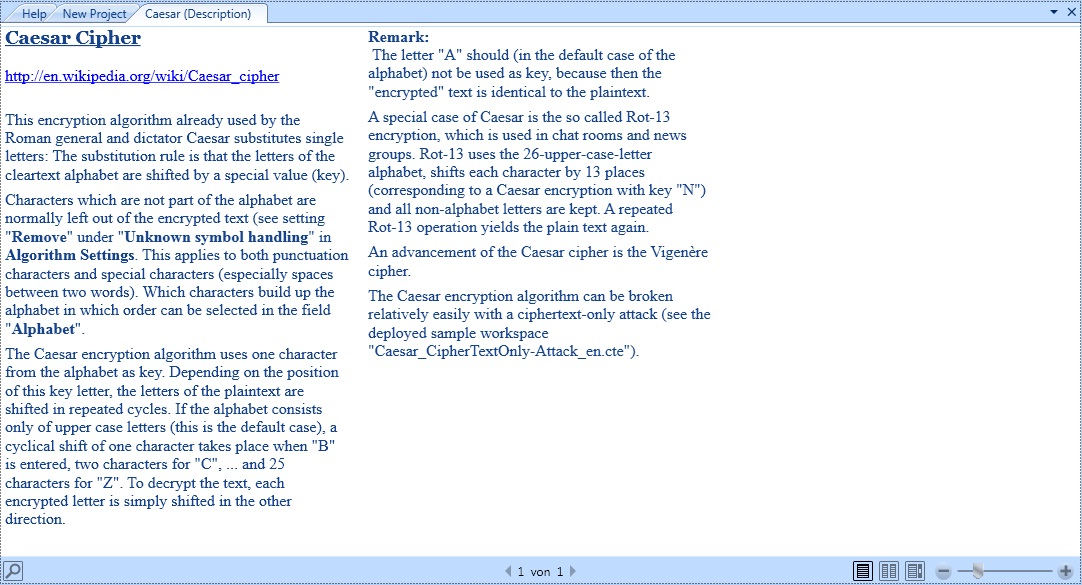
\includegraphics[width=1.00\textwidth]{figures/xaml_description.jpg}
	\caption{A detailed description provided through an XAML file.}
	\label{fig:xaml_description}
\end{figure}
\clearpage

The last parameter tells CrypTool 2 the names of the provided icons. This parameter is an array composed of strings in the format \textit{$<$assembly name$>$/$<$file name$>$} or \textit{$<$assembly name$>$/$<$path$>$/$<$file name$>$}.

The first and most important icon is the plugin icon, which will be shown in CrypTool 2 in the ribbon bar and navigation pane. Once the icon has been added to the project as described in Section \ref{sec:AddingAnIconToTheCaesarClass}, we must accordingly tell CrypTool 2 where to find the icon. This can be seen above in Figure \ref{fig:attribute_plugininfo}.

%\begin{figure}[h!]
%	\centering
%		
\includegraphics[width=1.00\textwidth]{figures/attribute_plugininfo_icons.jpg}
%	\caption{Attribute PluginInfo icons}
%	\label{fig:attribute_plugininfo_icons}
%\end{figure}

If your plugin will use additional icons, you should define the paths to each of them by adding the path strings to the \textit{[PluginInfo]} attribute parameter list, each separated by a comma. We have added two further icons for the context menu in the CrypTool 2 workspace. (If you do choose to add more icons, don't forget to add the icons to your solution.)

\subsection{The \protect\textit{[EncryptionType]} attribute}
\label{sec:TheEncryptionTypeAttribute}

The third and last attribute, \textit{[EncryptionType]}, is needed to tell CrypTool 2 what type of plugin we are creating. CrypTool 2 uses this information to place the plugin in the correct group in the navigation pane and ribbon bar. In our example, since Caesar is a classical algorithm, we will define the follows:

\begin{figure}[h]
	\centering
		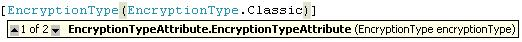
\includegraphics[width=.90\textwidth]{figures/attribute_encryptiontype_new.jpg}
	\caption{A fully-defined \textit{[EncryptionType]} attribute.}
	\label{fig:attribute_encryption_type}
\end{figure}

The possible values of the \textit{[EncryptionType]} attribute are as follows:

\begin{itemize}
	\item Asymmetric --- for asymmetrical encryption algorithms, such as RSA.
	\item SymmetricBlock --- for block cipher algorithms, such as DES, AES and Twofish.
	\item SymmetricStream --- for stream cipher algorithms, such as RC4, Rabbit and SEAL.
	\item Hybrid --- for algorithms which are actually a combination of several algorithms, such as algorithms in which the data is encrypted symmetrically and the encryption key asymmetrically.
	\item Classic --- for classical encryption or hash algorithms, such as Caesar or MD5.
\end{itemize}

\section{Defining the private variables of the settings in the Caesar class}
\label{sec:DefiningThePrivateVariablesOfTheSettingsInTheCaesarClass}

The next step is to define some private variables that are needed for the settings, input, and output data. In our example, this will look like the following:

\begin{lstlisting}
public class Caesar : IEncryption
{
	#region Private variables
	private CaesarSettings settings;
	private string inputString;
	private string outputString;
	private enum CaesarMode { encrypt, decrypt };
	private List<CryptoolStream> listCryptoolStreamsOut = new List<CryptoolStream>();
	#endregion
\end{lstlisting}

\ \\ % ugly but functional
If your algorithm works with longs strings of code, it is recommended to use the ``CryptoolStream'' data type. This was designed for input and output between plugins and to handle large amounts of data. To use the native CrypTool stream type, include the namespace ``Cryptool.PluginBase.IO'' with a ``using'' statement as explained in Section \ref{sec:AddingTheNamespacesAndInheritanceSourcesForTheCaesarClass}.

The following private variables will be used in our example:

\begin{itemize}
	\item CaesarSettings settings --- required to implement the IPlugin interface properly.
	\item string inputString --- string from which to read the input data.
	\item string outputString --- string to which to save the output data.
	\item enum CaesarMode --- used to select either encryption or decryption.
	\item List$<$CryptoolStream$>$ listCryptoolStreamsOut --- a list of all streams created by the plugin, which helps to perform a clean dispose.
\end{itemize}

\section{Implementing the interfaces in the Caesar class}
\label{sec:ImplementingTheInterfacesInTheCaesarClass}

The next major step is to write out our implementations of the interfaces. First we will add a constructor to our class. We will use this to create an instance of our settings class and a function to handle events:

\begin{lstlisting}
public class Caesar : IEncryption
{
	#region Private variables
	private CaesarSettings settings;
	private string inputString;
	private string outputString;
	private enum CaesarMode { encrypt, decrypt };
	private List<CryptoolStream> listCryptoolStreamsOut = new List<CryptoolStream>();
	#endregion
	
	public Caesar()
	{
		this.settings = new CaesarSettings();
		this.settings.LogMessage += Caesar_LogMessage;
	}
\end{lstlisting}

\ \\
\indent Secondly, we must implement the ``Settings'' property declared in the interface. An outline of this property should have been automatically generated by implementing the interface (see Section \ref{sec:AddingInterfaceFunctionsToTheCaesarClass}); just edit it appropriately to communicate with your settings class as we have done here:

\begin{lstlisting}
public ISettings Settings
{
	get { return (ISettings)this.settings; }
	set { this.settings = (CaesarSettings)value; }
}
\end{lstlisting}

\ \\
\indent Thirdly, we must define five properties, each with an appropriate attribute. This step is necessary to tell CrypTool 2 if the properties are used for input our output and to provide the plugin with external data.

The attribute that we will use for each proprerty is called \textit{[PropertyInfo]} and it consists of the following elements:

\begin{itemize}
	\item direction --- defines whether this property is an input or output property, e.g.\ whether it reads input data or writes output data. The possible values are:
	\begin{itemize}
		\item Direction.Input
		\item Direction.Output
	\end{itemize}
	\item caption --- the caption for the property displayed over the input of the icon after it has been placed in the editor), as seen below:
	
\begin{figure}[h]
	\centering
		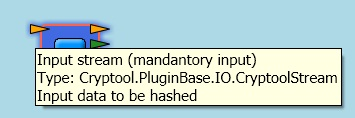
\includegraphics[width=.55\textwidth]{figures/property_caption.jpg}
	\caption{A possible property caption and toolTip.}
	\label{fig:property_caption}
\end{figure}

	\item toolTip --- the toolTip for the property displayed over the input arrow of the icon after it has been placed in the editor, as seen above.
	\item descriptionUrl --- currently not used; fill it with null or an empty string.
	\item mandatory --- this flag determines whether an input must be attached by the user to use the plugin. If set to true, an input connection will be required or else the plugin will not be executed in the workflow chain. If set to false, connecting an input is optional. As this only applies to input properties, if the direction has been set to ``output'', this flag will be ignored.
	\item hasDefaultValue --- if this flag is set to true, CrypTool 2 will assume that the property has a default input value that does not require user input.
	\item displayLevel --- determines in which display levels your property will be shown in CrypTool 2. These are used to hide more advanced item from less-experienced users; a beginner using the corresponding display level will not see the properties marked as any other level, but a professional using the appropriate display level will have access to everything. These levels are as follows:
	
	\begin{itemize}
		\item DisplayLevel.Beginner
		\item DisplayLevel.Experienced
		\item DisplayLevel.Expert
		\item DisplayLevel.Professional
	\end{itemize}
\clearpage
	
	\item quickWatchFormat --- determines how the content of the property will be shown in the quickwatch perspective. CrypTool accepts the following quickwatch formats:
	
	\begin{itemize}
		\item QuickWatchFormat.Base64
		\item QuickWatchFormat.Hex
		\item QuickWatchFormat.None
		\item QuickWatchFormat.Text
	\end{itemize}

\begin{figure}[h]
	\centering
		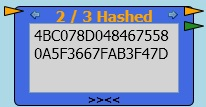
\includegraphics{figures/quick_watch.jpg}
	\caption{A quickwatch display in hexadecimal.}
	\label{fig:quick_watch}
\end{figure}
	
	\item quickWatchConversionMethod --- this is used to indicate a conversion method; most plugins do not ned to convert their data and thus should use a null value here. The quickwatch function uses the ``default'' system encoding to display data, so if your data is in another other format, such as Unicode or UTF-8, you should provide here the name of a conversion method as string. The method header for such a method should look something like the following:

\begin{lstlisting}
object YourMethodName(string PropertyNameToConvert)
\end{lstlisting}

\end{itemize}

The first of the five properties that we will define is ``InputString''. This is used to provide our plugin with the data to be encrypted or decrypted:

\begin{lstlisting}
[PropertyInfo(Direction.InputData, "Text input", "Input a string to be processed by the Caesar cipher", "", true, false, DisplayLevel.Beginner, QuickWatchFormat.Text, null)]
public string InputString
{
	get { return this.inputString; }
	set
  {
		if (value != inputString)
		{
			this.inputString = value;
			OnPropertyChanged("InputString");
		}
	}
}
\end{lstlisting}

In the get method we simply return the value of the input data. The set method checks if the input value has changed, and, if so, sets the new input data and announces the change to the CrypTool 2 environment by calling the function ``OnPropertyChanged(\textit{$<$Property name$>$})''. This step is necessary for input properties to update the quickwatch view.
\clearpage

%\textit{\small Note 1: It is currently not possible to read directly from the input data stream without creating an intermediate CryptoolStream.\\\\
%\small Note 2: The naming may be confusing. The new CryptoolStream is not an output stream, but it is added to the list of output streams to enable a clean dispose afterwards. See chapter 9 below.\\\\}

The output data property (which handles the input data after it has been encrypted or decrypted) will in our example look as follows:

\begin{lstlisting}
[PropertyInfo(Direction.OutputData, "Text output", "The string after processing with the Caesar cipher", "", false, false, DisplayLevel.Beginner, QuickWatchFormat.Text, null)]
public string OutputString
{
	get { return this.outputString; }
	set
	{
		outputString = value;
		OnPropertyChanged("OutputString");
	}
}
\end{lstlisting}

\ \\
\indent CrypTool 2 does not require implementing output set methods, as they will never be called from outside the plugin. Nevertheless, in our example the plugin accesses the property itself, and therefore we have chosen to implement the set method.

You can provide additional output data types if you so desire. In our example, we will also offer output data of type CryptoolStream, input data for external alphabets, and input data for the shift value of our Caesar algorithm. Note that for the first of these, the set method is not implemented since it will never be called. We shall define these properties as follows:

\begin{lstlisting}
[PropertyInfo(Direction.OutputData, "propStreamOutputToolTip", "propStreamOutputDescription", "", false, false, DisplayLevel.Beginner, QuickWatchFormat.Text, null)]
public CryptoolStream OutputData
{
	get
	{
		if (outputString != null)
		{
			CryptoolStream cs = new CryptoolStream();
			listCryptoolStreamsOut.Add(cs);
			cs.OpenRead(Encoding.Default.GetBytes(outputString.ToCharArray()));
			return cs;
		}
		else
		{
			return null;
		}
	}
	set { }
}

[PropertyInfo(Direction.InputData, "External alphabet input", "Input a string containing the alphabet to be used by Caesar.\nIf no alphabet is provided for this input, the internal default alphabet will be used.", "", false, false, DisplayLevel.Expert, QuickWatchFormat.Text, null)]
public string InputAlphabet
{
	get { return ((CaesarSettings)this.settings).AlphabetSymbols; }
	set
	{
		if (value != null && value != settings.AlphabetSymbols)
		{
			((CaesarSettings)this.settings).AlphabetSymbols = value;
			OnPropertyChanged(''InputAlphabet'');
		}
	}
}

[PropertyInfo(Direction.InputData, "Shift value (integer)", "This is the same setting as the shift value in the Settings pane but as dynamic input.", "", false, false, DisplayLevel.Expert, QuickWatchFormat.Text, null)]
public int ShiftKey
{
	get { return settings.ShiftKey; }
	set
	{
		if (value != settings.ShiftKey)
		{
			settings.ShiftKey = value;
		}
	}
}
\end{lstlisting}

\ \\
\indent The CrypTool 2 API provides two methods to send messages from the plugin to the CrypTool 2 core: ``GuiLogMessage'' (used to send messages to the CrypTool 2 status bar) and ``OnPropertyChanged'' (used to inform the core of changes to the plugin data). The ``GuiLogMessage'' method is a nice mechanism to inform the user as to what your plugin is currently doing.

\begin{figure}[h]
	\centering
		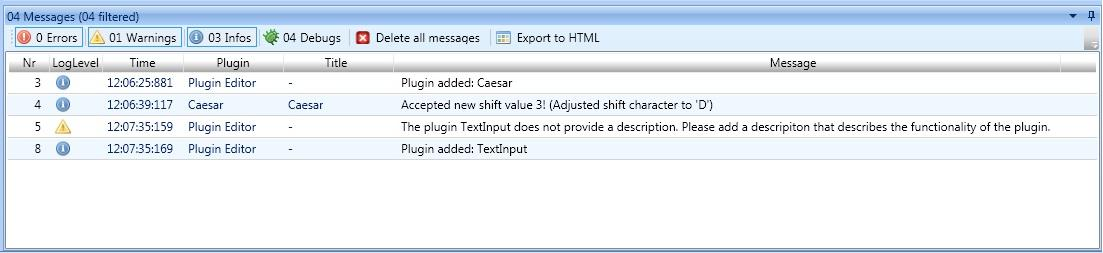
\includegraphics[width=1.00\textwidth]{figures/status_bar.jpg}
	\caption{An example status bar.}
	\label{fig:status_bar}
\end{figure}
\clearpage

The method takes two parameters:

\begin{itemize}
	\item Message --- the text (of type string) to be shown in the status bar.
	\item NotificationLevel --- the type of message, that is, its alert level:
	\begin{itemize}
		\item NotificationLevel.Error
		\item NotificationLevel.Warning
		\item NotificationLevel.Info
		\item NotificationLevel.Debug
	\end{itemize}
\end{itemize}

Outlines of both of the related events will have been automatically generated by implementing the interface (see Section \ref{sec:AddingInterfaceFunctionsToTheCaesarClass}), but we must define appropriate methods as follows:

\begin{lstlisting}
public event GuiLogNotificationEventHandler OnGuiLogNotificationOccured;
private void GuiLogMessage(string message, NotificationLevel logLevel)
{
	EventsHelper.GuiLogMessage(OnGuiLogNotificationOccured, this, new GuiLogEventArgs(message, this, logLevel));
}

public event PropertyChangedEventHandler PropertyChanged;

public void OnPropertyChanged(String name)
{
	EventsHelper.PropertyChanged(PropertyChanged, this, new PropertyChangedEventArgs(name));
}
\end{lstlisting}

\ \\
\indent Note that to use ``PropertyChangedEventHandler'' you must include the namespace ``System.\linebreak ComponentModel''. Our collection of included namespaces should now look as follows:

\begin{lstlisting}
using System.Collections.Generic;
using System.Text;
using System.ComponentModel;
using System.Windows.Controls;

using Cryptool.PluginBase;
using Cryptool.PluginBase.Cryptography;
using Cryptool.PluginBase.IO;
using Cryptool.PluginBase.Miscellaneous;
\end{lstlisting}
\clearpage

\section{Completing the algorithmic code of the Caesar class}
\label{sec:CompletingTheAlgorithmicCodeOfTheCaesarClass}

At this point, the plugin should be ready to be read by and shown correctly in the CrypTool 2 application. However, we haven't actually implemented the algorithm yet. This should be done in the ``Execute()'' function, as this is what CrypTool 2 will always call first. The actual functionality of your algorithm, as well as the structure thereof, is up to you. Note that an outline of the ``Execute()'' function will have been automatically generated by implementing the interface (see Section \ref{sec:AddingInterfaceFunctionsToTheCaesarClass}).

We have chosen to split our algorithm's encryption and decryption into two separate functions, which will both ultimately call the ``ProcessCaesar()'' function. Below is our implementation of the Execute() function:

\begin{lstlisting}
private void ProcessCaesar(CaesarMode mode)
{
	CaesarSettings cfg = (CaesarSettings)this.settings;
	StringBuilder output = new StringBuilder("");
	string alphabet = cfg.AlphabetSymbols;

	// In case we are working in case-insensitive mode, we will use
	// only capital letters, hence we must transform the whole alphabet
	// to uppercase.
	if (!cfg.CaseSensitiveAlphabet)
	{
		alphabet = cfg.AlphabetSymbols.ToUpper();
	}

	if (inputString != null)
	{
		for (int i = 0; i < inputString.Length; i++)
		{
			// Get the plaintext char currently being processed.
			char currentchar = inputString[i];

			// Store whether it is upper case (otherwise lowercase is assumed).
			bool uppercase = char.IsUpper(currentchar);

			// Get the position of the plaintext character in the alphabet.
			int ppos = 0;
			if (cfg.CaseSensitiveAlphabet)
			{
				ppos = alphabet.IndexOf(currentchar);
			}
			else
			{
				ppos = alphabet.IndexOf(char.ToUpper(currentchar));
			}

			if (ppos >= 0)
			{
				// We found the plaintext character in the alphabet,
				// hence we will commence shifting.
				int cpos = 0;
				switch (mode)
				{
					case CaesarMode.encrypt:
						cpos = (ppos + cfg.ShiftKey) % alphabet.Length;
						break;
					case CaesarMode.decrypt:
						cpos = (ppos - cfg.ShiftKey + alphabet.Length) % alphabet.Length;
						break;
				}

				// We have the position of the ciphertext character,
				// hence just output it in the correct case.
				if (cfg.CaseSensitiveAlphabet)
				{
					output.Append(alphabet[cpos]);
				}
				else
				{
					if (uppercase)
					{
						output.Append(char.ToUpper(alphabet[cpos]));
					}
					else
					{
						output.Append(char.ToLower(alphabet[cpos]));
					}
				}
			}
			else
			{
				// The plaintext character was not found in the alphabet,
				// hence proceed with handling unknown characters.
				switch ((CaesarSettings.UnknownSymbolHandlingMode)cfg.UnknownSymbolHandling)
				{
					case CaesarSettings.UnknownSymbolHandlingMode.Ignore:
						output.Append(inputString[i]);
						break;
					case CaesarSettings.UnknownSymbolHandlingMode.Replace:
						output.Append('?');
						break;
				}
			}

			// Show the progress.
			if (OnPluginProgressChanged != null)
			{
				OnPluginProgressChanged(this, new PluginProgressEventArgs(i, inputString.Length - 1));
			}
		}
		outputString = output.ToString();
		OnPropertyChanged("OutputString");
		OnPropertyChanged("OutputData");
	}
}

public void Encrypt()
{
	ProcessCaesar(CaesarMode.encrypt);
}

public void Decrypt()
{
	ProcessCaesar(CaesarMode.decrypt);
}

public void Execute()
{
	switch (settings.Action)
	{
		case 0:
			Caesar_LogMessage("Encrypting", NotificationLevel.Debug);
			Encrypt();
			break;
		case 1:
			Caesar_LogMessage("Decrypting", NotificationLevel.Debug);
			Decrypt();
			break;
		default:
    	break;
	}
}
\end{lstlisting}

It is important to make sure that all changes to the output properties will be announced to the CrypTool 2 environment. In our example this happens by calling the set method of OutputData, which in turn calls ``OnPropertyChanged'' for both output properties ``OutputData'' and ``OutputDataStream''. Instead of calling the property's set method you can instead call ``OnPropertyChanged'' directly within the ``Execute()'' method.\clearpage

You have probably noticed that the ``ProgressChanged'' method is undefined. This can be used to show the current algorithm process as a progress bar in the plugin icon. To use this method and compile successfully, you must declare this method, as we have done for our example below:

\begin{lstlisting}
public event PluginProgressChangedEventHandler OnPluginProgressChanged;
private void ProgressChanged(double value, double max)
{
	EventsHelper.ProgressChanged(OnPluginProgressChanged, this, new PluginProgressEventArgs(value, max));
}
\end{lstlisting}

\section{Performing a clean dispose}
\label{sec:PerformingACleanDispose}

Be sure you have closed and cleaned all your streams after execution before CrypTool 2 decides to dispose the plugin instance. Though not required, we will run the disposal code before execution as well. We will expand the associated automatically generated methods (see Section \ref{sec:AddingInterfaceFunctionsToTheCaesarClass}) as follows:

\begin{lstlisting}
public void Dispose()
{
	foreach(CryptoolStream stream in listCryptoolStreamOut)
	{
		stream.Close();
	}
	listCryptoolStreamOut.Clear();
}

public void PostExecution()
{
	Dispose();
}

public void PreExecution()
{
	Dispose();
}
\end{lstlisting}
\clearpage

\section{Finishing the implementation}
\label{sec:FinishingTheImplementation}

When adding plugin instances to the CrypTool 2 workspace, the application core checks whether the plugin runs without any exceptions. If any method inherited from IPlugin throws an exception, CrypTool 2 will display an error message and prohibit use of the plugin. Therefore, we must remove the ``NotImplementedException'' from the automatically generated methods ``Initialize()'', ``Pause()'' and ``Stop()''. In our example it will be sufficient to provide empty implementations.

\begin{lstlisting}
public void Initialize()
{
}

public void Pause()
{
}

public void Stop()
{
}
\end{lstlisting}

The methods ``Presentation()'' and ``QuickWatchPresentation()'' can be used to provide a specialized visualization of the plugin algorithm to be shown in CrypTool. Take a look at the ``PRESENT'' plugin to see how a custom visualization can be realized. For our Caesar example, we have chosen not to implement a custom visualization. Therefore we will simply return ``null'':

\begin{lstlisting}
public UserControl Presentation
{
	get { return null; }
}

public UserControl QuickWatchPresentation
{
	get { return null; }
}
\end{lstlisting}

Your plugin should compile without errors at this point.
\clearpage

\section{Importing and testing the plugin}
\label{sec:ImportingAndTestingThePlugin}

After you have built the plugin, you need to move the newly created plugin DLL to a location where CrypTool 2 can find it. There are a few different ways to accomplish this. You can find the DLL file in \textit{\textbackslash CrypPluginBase\textbackslash bin\textbackslash Debug}.

\subsection{Global storage}
\label{sec:GlobalStorage}

The first option is to copy your plugin's DLL file to the ``CrypPlugins'' folder in which the CrypTool 2 executable (``CrypWin.exe'') can be found. %If necessary, create the folder ''CrypPlugins''.

\begin{figure}[h]
	\centering
		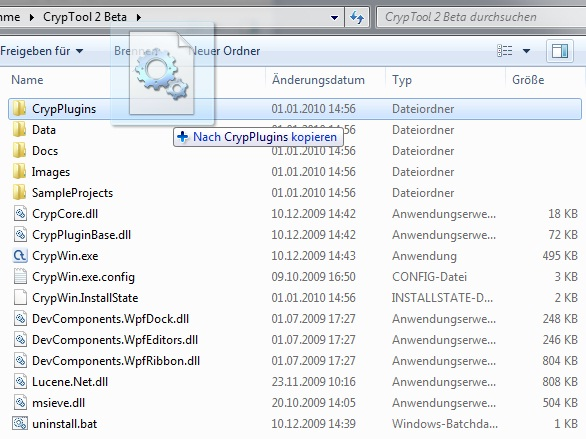
\includegraphics{figures/copy_dll_global_storage.jpg}
	\caption{Copying the plugin to the global storage folder}
	\label{fig:copy_dll_global_storage}
\end{figure}

This folder is known as ``global storage'' in the CrypTool 2 architecture. Changes in this folder will affect all users on a multi-user Windows platform. You should now restart CrypTool 2.
\clearpage

\begin{figure}[h]
	\centering
		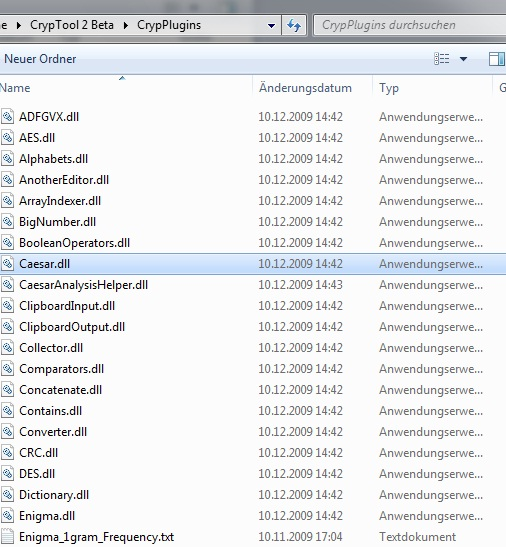
\includegraphics{figures/global_storage.jpg}
	\caption{Inside the CrypPlugins folder (the global storage).}
	\label{fig:global_storage}
\end{figure}

\subsection{Custom storage}
\label{sec:CustomStorage}

The second possibility is to copy your plugin's DLL file to the ``CrypPlugins'' folder located in the ``Application Data'' folder in your home folder. In Windows XP, the home folder path should be as follows: \textit{C:\textbackslash Documents and Settings\textbackslash $<$user name$>$\textbackslash Application Data\textbackslash CrypPlugins}, and in Vista and Windows 7 the path should look like: \textit{C:\textbackslash Users\textbackslash $<$user name$>$\textbackslash Application Data\textbackslash CrypPlugins}. This home folder path is called ``custom storage'' in the CrypTool architecture. Changes in this folder will only take effect for current user. After copying the file, you must restart CrypTool 2.
\clearpage

\begin{figure}[h]
	\centering
		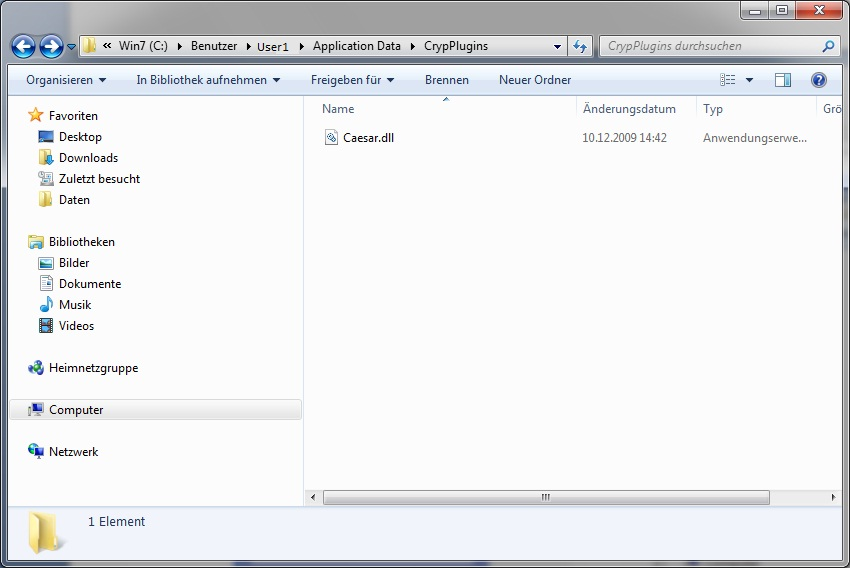
\includegraphics[width=1.00\textwidth]{figures/custom_storage.jpg}
	\caption{The custom storage folder.}
	\label{fig:custom_storage}
\end{figure}

\subsection{Importing directly}
\label{sec:ImportingDirectly}

Alternatively, you can import new plugins directly from the CrypTool 2 interface. Just run \mbox{CrypWin.exe} and select the ``Download Plugins'' button. An ``Open File Dialog'' window will open and ask where the new plugin is located. After selecting the new plugin, CrypTool 2 will automatically import the plugin to the custom storage folder. With this option you will not have to restart the program. All corresponding menu entries will be updated automatically. Note that this import function only accepts \textbf{signed} plugins, and also that this option is just a temporary solution: in the future this will be done online by a web service.
\clearpage

\subsection{Using build settings}
\label{sec:UsingBuildSettings}

Yet another option is to use the build settings in your plugin's project properties to copy the DLL automatically after building it in Visual Studio. To set this up, right-click on your plugin project and select ``Properties'':

\begin{figure}[h]
	\centering
		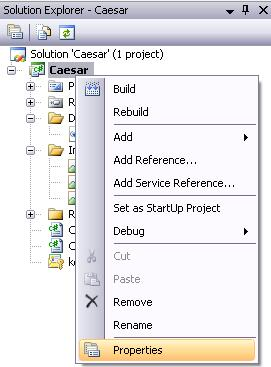
\includegraphics{figures/solution_properties.JPG}
	\caption{Selecting the solution properties.}
	\label{fig:solution_properties}
\end{figure}
\clearpage

\noindent Then select ``Build Events'':

\begin{figure}[h]
	\centering
		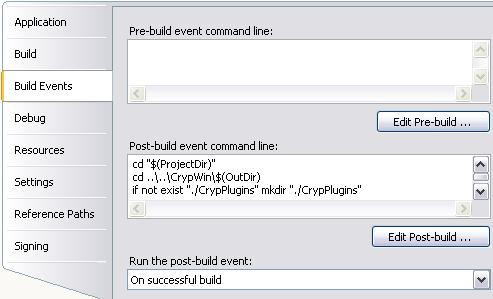
\includegraphics{figures/post_build.JPG}
	\caption{Setting the build events.}
	\label{fig:post_build}
\end{figure}

\noindent And finally, enter the following text into ``Post-build event command line'':\\\\
cd "\$(ProjectDir)" \\
cd ..\textbackslash ..\textbackslash CrypWin\$(OutDir)\\
if not exist "./CrypPlugins" mkdir "./CrypPlugins"\\
del /F /S /Q /s /q "\fcolorbox{yellow}{yellow}{Caesar}*.*"\\
copy "\$(TargetDir)\fcolorbox{yellow}{yellow}{Caesar}*.*" "./CrypPlugins"\\\\
You will need to change the marked fields to your particular plugin's name.

\section{Downloading the example and template}
\label{sec:DownloadingTheExampleAndTemplate}

If you didn't download the entire CrypTool 2 source code as described in Section \ref{TheCrypTool2SVNURL}, but you want a copy of the source code for the Caesar algorithm that was used as an example in this guide, you can download it as a Visual Studio \textbf{solution} from the following location:\\\\
\textit{username: anonymous\\
password:} (not required)\\
\url{https://www.cryptool.org/svn/CrypTool2/trunk/CrypPlugins/Caesar/}\\\\
We have also created a Visual Studio plugin template to help with the development of new plugins. This can be found here:\\\\
\url{http://cryptool2.vs.uni-due.de/downloads/template/encryptionplugin.zip}
\clearpage

\section{Drawing the workflow of your plugin}
\label{DrawingTheWorkfloweOfYourPlugin}

Each plugin should have an associated workflow file to show the algorithm in action in CrypTool 2. Such a file can be automatically created by simply saving a CrypTool 2 workspace project featuring your plugin. Below is a possible workflow for our Caesar example:

\begin{figure}[h]
	\centering
		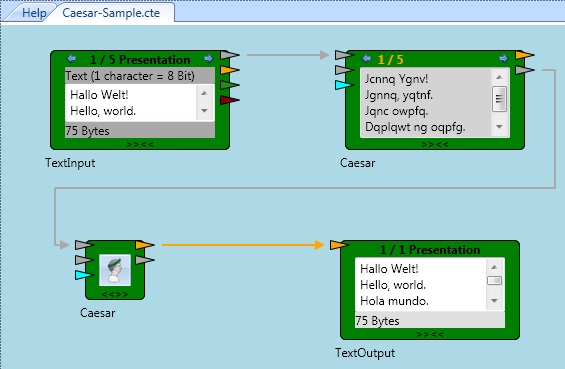
\includegraphics{figures/sample.jpg}
	\caption{A sample workflow diagram for the Caesar algorithm.}
	\label{fig:sample}
\end{figure}

\end{document}
